\documentclass[12pt,xcolor=table,aspectratio=169]{beamer}
\usetheme{Frankfurt}
\usecolortheme{rose}
\usepackage{amsthm}
\usepackage{amsmath}
\usepackage{bbm}
\usepackage{amsfonts}
\usepackage{amssymb}
\usepackage{graphicx}
\usepackage{hyperref}
\usepackage[flushleft]{threeparttable}
\usepackage{tabularx}
\usepackage{booktabs}
\usepackage{siunitx}
\usepackage{tikz}
\usetikzlibrary{decorations.pathreplacing,angles,quotes}
%\usepackage{enumitem}% http://ctan.org/pkg/enumitem

%set up course and number

\newcommand{\ClassName}{TBD}
\newcommand{\ClassNumber}{TBD}
\newcommand{\Topic}{TBD}

% Some optional colors. Change or add as you see fit.
%---------------------------------------------------
 \definecolor{ualbertagreen}{HTML}{007C41}
\definecolor{ualbertagold}{HTML}{FFDB05}

\definecolor{calloutgrey}{HTML}{D9D9D9}


%set fonts
\setbeamerfont{subtitle}{size=\large,shape=\scshape,series=\bfseries}
\setbeamerfont{title}{size=\Large,shape=\scshape,series=\bfseries}
\setbeamerfont{author}{size=\large}
\setbeamerfont{date}{size=\large}
\setbeamerfont{caption}{size=\scriptsize}


% Some optional color adjustments to Beamer. Change as you see fit.
%------------------------------------------------------------------
\setbeamercolor{frametitle}{fg=ualbertagreen,bg=white}
\setbeamercolor{title}{fg=ualbertagreen,bg=white}
\setbeamercolor{author}{fg=ualbertagreen,bg=white}
\setbeamercolor{date}{fg=ualbertagreen,bg=white}
\setbeamercolor{local structure}{fg=ualbertagreen}
\setbeamercolor{section in toc}{fg=ualbertagreen,bg=white}
% \setbeamercolor{subsection in toc}{fg=ualbertagreen,bg=white}
\setbeamercolor{footline}{fg=ualbertagreen!50, bg=white}

% definition boxes
\setbeamercolor{block title}{bg=ualbertagreen,fg=white}
\setbeamercolor{block body}{parent=normal text,use=block title,bg=calloutgrey}
%\setbeamercolor{block body}{parent=normal text,use=block title,bg=block title.bg!30!bg}


\setbeamercolor{upper separation line head}{bg=ualbertagreen}
\setbeamercolor{lower separation line head}{bg=ualbertagold}
\setbeamercolor{middle separation line head}{bg=ualbertagold}
\setbeamercolor{frametitle}{fg=ualbertagreen,bg=white}



\setbeamercolor{section in head/foot}{bg=white,fg=ualbertagreen}
\setbeamercolor{author in head/foot}{bg=white,fg=ualbertagreen}
\setbeamercolor{date in head/foot}{bg=white,,fg=ualbertagreen}
\setbeamercolor{title in head/foot}{bg=white,fg=ualbertagreen}

\setbeamercolor{headline}{bg=white,fg=ualbertagreen}




\setbeamercolor*{middle separation line head}{bg=ualbertagreen}
\setbeamercolor*{alerted text}{fg=ualbertagreen}
\setbeamercolor*{example text}{fg=black}
\setbeamercolor*{structure}{fg=black}


\let\Tiny=\tiny



\logo{
   %\ifnum\insertpagenumber>1
   \tikz [remember picture,overlay]
    \node[yshift=.3cm,xshift=1.5cm] at (current page.south west)
        %or: (current page.center)
        {
\includegraphics[width=1in]{../images/UA-ASB-COLOUR.png}};
    %\fi
%
\includegraphics[height=0.8cm]{../images/UA-ASB-COLOUR.png}\vspace{220pt}
}


\setbeamertemplate{title page}{%
  \vbox{}
    \vspace{.5cm}% NEW
  \begingroup
    \centering
    \begin{beamercolorbox}[sep=8pt,center]{title}
      \usebeamerfont{title}\ClassNumber: \ClassName\par%
      \usebeamerfont{title}\inserttitle\par%
     \ifx\insertsubtitle\@empty%
      \else%
        \vskip0.05em%
        {\usebeamerfont{subtitle}\usebeamercolor[fg]{subtitle}\insertsubtitle\par}%
      \fi%
    \end{beamercolorbox}%
    \begin{beamercolorbox}[sep=8pt,center]{author}
      \usebeamerfont{author}\insertauthor
    \end{beamercolorbox}
    \begin{beamercolorbox}[sep=8pt,center]{institute}
      \usebeamerfont{institute}\insertinstitute
    \end{beamercolorbox}

    \vspace{0.5cm}% NEW
    \begin{beamercolorbox}[sep=8pt,center]{date}
      \usebeamerfont{date}\insertdate
    \end{beamercolorbox}\vskip0.05em

      \endgroup
  %\vfill
}


\setbeamertemplate{frametitle}{%
    \insertframetitle\par\vskip-10pt
}



\renewcommand{\ClassName}{Business Economics, Organization and Management}
\renewcommand{\ClassNumber}{BUEC 311}

\setbeamertemplate{headline}{%
\leavevmode%
 \hbox{%
    \begin{beamercolorbox}[wd=\paperwidth,ht=5ex,dp=0ex]{white}%
    \usebeamerfont{headline}\hskip6pt\ClassNumber: \inserttitle\par%
    \insertsectionnavigationhorizontal{\paperwidth}{}{\hskip0pt plus1filll}
    \end{beamercolorbox}%
  }
}

\defbeamertemplate*{footline}{my footline}{%
    \ifnum\insertpagenumber=1
        \Tiny{%
            \hfill%
		\vspace*{1pt}%
            %\insertframenumber/\inserttotalframenumber \hspace*{0.1cm}%
            \newline%
            \color{ualbertagold}{\rule{\paperwidth}{0.4mm}}\newline%
            \color{ualbertagold}{\rule{\paperwidth}{.4mm}}%
        }
  \else%
        \Tiny{%
            \hspace{.66\paperwidth}
            %\vspace{25pt}
            \insertframenumber/\inserttotalframenumber
            \newline%
            \color{ualbertagold}{\rule{\paperwidth}{0.4mm}}\newline%
            \color{ualbertagold}{\rule{\paperwidth}{.4mm}}%
        }%
    \fi%
}


\newenvironment{itemize*}%
  {\begin{itemize}%
    \setlength{\itemsep}{0pt}%
    \setlength{\parskip}{0pt}}%
  {\end{itemize}}



\title{Consumer Behaviour}

\date{Fall 2020}

\begin{document}


\frame{
	\titlepage
}

\section{Outline}

\frame{
	\frametitle{Outline}
	\begin{enumerate}
	\item Motivation: Consumer decision making
	\item[]
	\item The theory of consumer choice.
		\begin{itemize}
		\item Preferences and utility.
		\item The budget constraint.
		\item Determining consumer choice.
		\end{itemize}
	\item[]
	\item Applying the theory.
		\begin{itemize}
		\item Designing promotions.
		\item Deriving demand curves.
		\end{itemize}
	\item[]
	\item Deviations from the theory.
		\begin{itemize}
		\item Behavioural economics.
		\end{itemize}
	\end{enumerate}
}

\frame{
	\frametitle{Motivation: Consumer Decision Making.}
	\begin{itemize}
	\item How do you decide to buy the things that you do?
	\end{itemize}
}

\section{Consumer Choice Theory}


\frame{
	\frametitle{The Theory of Consumer Choice}
	\begin{itemize}
	\item One possible explanation for consumer choice: random decision making.
		\begin{itemize}
		\item Consumers act blindly and make decisions without any thought.
		\end{itemize}
	\item[]
	\item An alternative explanation for consumer choice: individuals make systematic decisions.
		\begin{itemize}
		\item But then, what drives systematic decision making?
		\end{itemize}
	\end{itemize}
}	

\frame{
	\frametitle{The Theory of Consumer Choice}
	\begin{itemize}
	\item Economists rely on the \textit{Theory of Consumer Choice} to understand how consumers make decisions.
	\item[]
	\item This model of behaviour relies on three main premises.
		\begin{enumerate}
		\item Consumers have \textit{preferences} that determine the satisfaction they get from the consumption of goods and services.
		\item Consumers face \textit{constraints} that limit their choices.
		\item Consumers seek to \textit{maximize} the level of satisfaction they obtain from consumption given the constraints that they face.
		\end{enumerate}
	\end{itemize}
}

\frame{
	\frametitle{The Theory of Consumer Choice: Preferences}
	\begin{itemize}
	\item Economists assume that consumers have a set of \textit{tastes} or \textit{preferences} that they use to guide them in choosing between goods.
	\item[]
	\item These tastes may differ substantially among individuals due to differences in culture, experience, etc.
		\begin{itemize}
		\item E.g. Hershey's chocolate.
		\end{itemize}
	\end{itemize}
}

\frame{
	\frametitle{The Theory of Consumer Choice: Preferences}
	\begin{itemize}
	\item The standard model of consumer behaviour assumes preferences satisfy three key conditions:
		\begin{enumerate}
		\item Completeness
		\item Transitivity
		\item More is Better (Non-satiation)
		\end{enumerate}
	\item[]
	\item With these three properties, we can say a lot about how consumers make decisions.
	\end{itemize}
}

\frame{
	\frametitle{Condition 1: Completeness}
	\begin{itemize}
	\item \underline{Completeness}: Requires that for a consumer facing a choice between any two bundles of goods, $A$ and $B$, then either:
		\begin{itemize}
		\item The consumer prefers $A$ to $B$.
		\item The consumer prefers $B$ to $A$.
		\item The consumer is indifferent between $A$ and $B$.
		\end{itemize}
	\item[]
	\item This condition ensures that consumers can rank \textit{all possible bundles of goods} in terms of their desirability.
		\begin{itemize}
		\item Implication: consumers must be able to decide on preferences for all possible options; indecision is not possible.
		\item Is this reasonable?
		\end{itemize}
	\end{itemize}
}

\frame{
	\frametitle{Condition 2: Transitivity}
	\begin{itemize}
	\item \underline{Transitivity}: Requires that if a consumer strictly prefers $A$ to $B$, and strictly prefers $B$ to $C$, then they also strictly prefer $A$ to $C$.
	\item[]
	\item Also applies to weak preferences and indifference relationships.
	\item[]
	\item Transitivity ensures that individuals are rational in their choices.
		\begin{itemize}
		\item But are people rational?
		\end{itemize}
	\end{itemize}
}

\frame{
	\frametitle{Condition 3: More is Better}
	\begin{itemize}
	\item \underline{More is Better:} Requires that consumers always prefer more of a good to less.
	\item[]
	\item Condition is also referred to as ``non-satiation''.
	\item[]
	\item Do people always want more?
	\end{itemize}
}

\frame{
	\frametitle{The Theory of Consumer Choice: Preferences}
	\begin{itemize}
	\item The three conditions are very useful for understanding how consumers make decisions.
	\item[]
	\item To see this, consider the case of Taylor, who loves fast food.
	\item[]
	\item Taylor has to decide how many Burgers ($B$) and Tacos ($T$) to consume per month.
	\end{itemize}
}

\frame{
	\frametitle{The Theory of Consumer Choice: Preferences}

	\begin{figure}[t!]
	\center
	\resizebox{!}{.45\linewidth}{

	\begin{tikzpicture}
	% Draw axes
	%Y
	\draw[->] (0,0) -- (0,12) ;
	\draw[] (0,8) -- node[rotate=90, above=30pt] {\textbf{$B$, Burgers per month}} (0,10);
	%X
	\draw[->] (0,0) -- (15,0);
	\draw[] (14,0) -- node[below=30pt] {\textbf{$T$, Tacos per month}} (14,0);

	%Plot possible consumption bundles:
	%a
	\draw[fill] (8,6) circle [radius =0.1];
	\node at (8,6.1) [above] {{a}};
	%b
	\draw[fill] (4,2) circle [radius =0.1];
	\node at (4,2.1) [above] {{b}};	
	%c
	\draw[fill] (6,10) circle [radius =0.1];
	\node at (6,10.1) [above] {{c}};
	%d
	\draw[fill] (12,8) circle [radius =0.1];
	\node at (12,8.1) [above] {{d}};
	%e
	\draw[fill] (10,4) circle [radius =0.1];
	\node at (10,4.1) [above] {{e}};
	%5
	\draw[fill] (11,5) circle [radius =0.1];
	\node at (11,5.1) [above] {{f}};

	%Plot illustrative lines
%	\draw[dashed] (0,3) -- (8,3) -- (8,0);

	%Add axes labels
	%Origin%
	\node at (0,0) [left] {{0}};
	%Y Axis
	\node at (0,2) [left] {{2}};
	\node at (0,4) [left] {{4}};
	\node at (0,6) [left] {{6}};
	\node at (0,8) [left] {{8}};
	\node at (0,10) [left] {{10}};

	%X Axis
	\node at (2,0) [below] {{2}};
	\node at (4,0) [below] {{4}};
	\node at (6,0) [below] {{6}};
	\node at (8,0) [below] {{8}};
	\node at (10,0) [below] {{10}};
	\node at (12,0) [below] {{12}};
	\node at (14,0) [below] {{14}};


\end{tikzpicture}
}
\caption{Taylor's Possible Choices}
\end{figure}
}

\frame{
	\frametitle{The Theory of Consumer Choice: Preferences}
	\begin{itemize}
	\item Which bundles are preferred to $a$?
	\end{itemize}
}

\frame{
	\frametitle{The Theory of Consumer Choice: Preferences}
		%	The demand for cheese:
	
	\begin{figure}[t!]
	\center
	\resizebox{!}{.45\linewidth}{

	\begin{tikzpicture}
	% Draw axes
	%Y
	\draw[->] (0,0) -- (0,12) ;
	\draw[] (0,8) -- node[rotate=90, above=30pt] {\textbf{$B$, Burgers per month}} (0,10);
	%X
	\draw[->] (0,0) -- (15,0);
	\draw[] (14,0) -- node[below=30pt] {\textbf{$T$, Tacos per month}} (14,0);

	%Plot possible consumption bundles:
	%a
	\draw[fill, red] (8,6) circle [radius =0.1];
	\node at (8,6.1) [above] {{a}};
	%b
	\draw[fill] (4,2) circle [radius =0.1];
	\node at (4,2.1) [above] {{b}};	
	%c
	\draw[fill] (6,10) circle [radius =0.1];
	\node at (6,10.1) [above] {{c}};
	%d
	\draw[fill] (12,8) circle [radius =0.1];
	\node at (12,8.1) [above] {{d}};
	%e
	\draw[fill] (10,4) circle [radius =0.1];
	\node at (10,4.1) [above] {{e}};
	%5
	\draw[fill] (11,5) circle [radius =0.1];
	\node at (11,5.1) [above] {{f}};

	%Plot illustrative lines
%	\draw[dashed] (0,3) -- (8,3) -- (8,0);

	%Add axes labels
	%Origin%
	\node at (0,0) [left] {{0}};
	%Y Axis
	\node at (0,2) [left] {{2}};
	\node at (0,4) [left] {{4}};
	\node at (0,6) [left] {{6}};
	\node at (0,8) [left] {{8}};
	\node at (0,10) [left] {{10}};

	%X Axis
	\node at (2,0) [below] {{2}};
	\node at (4,0) [below] {{4}};
	\node at (6,0) [below] {{6}};
	\node at (8,0) [below] {{8}};
	\node at (10,0) [below] {{10}};
	\node at (12,0) [below] {{12}};
	\node at (14,0) [below] {{14}};


\end{tikzpicture}
}
\caption{Taylor's Possible Choices}
\end{figure}
}

\frame{
	\frametitle{The Theory of Consumer Choice: Preferences}
	\begin{itemize}
	\item We can use the three conditions to understand which bundles are preferred to $a$.
	\item[]
	\item First: More is better.
	\end{itemize}
}

\frame{
	\frametitle{The Theory of Consumer Choice: Preferences}
	
	\begin{figure}[t!]
	\center
	\resizebox{!}{.45\linewidth}{

	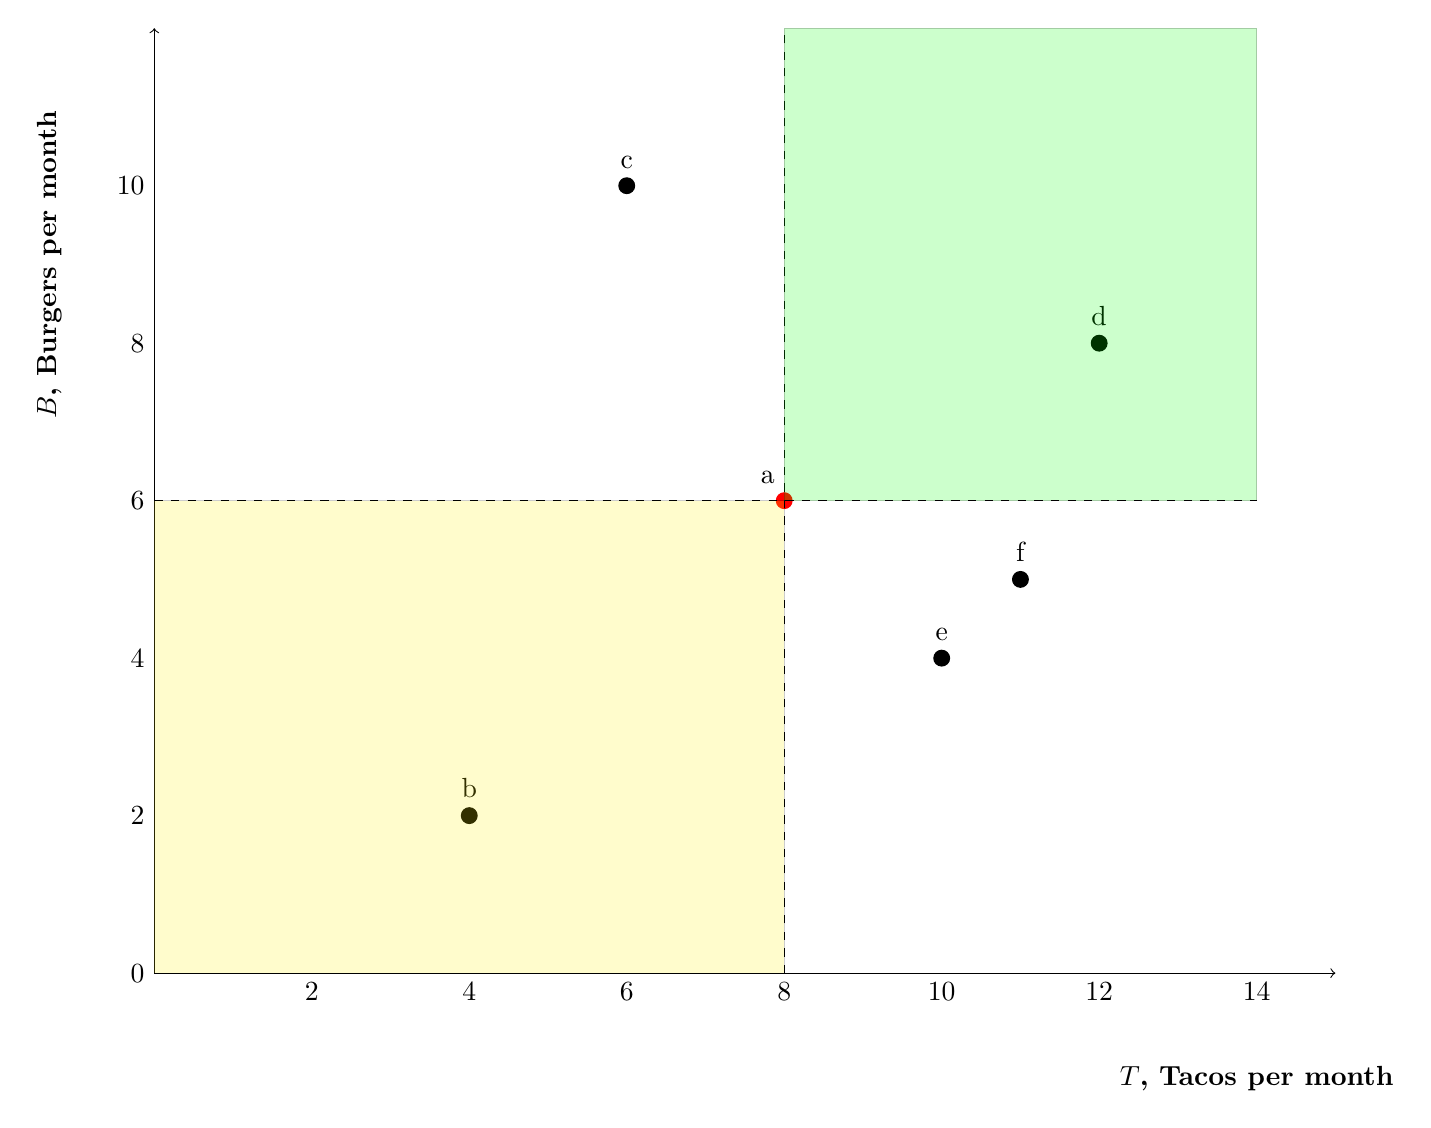
\begin{tikzpicture}
	% Draw axes
	%Y
	\draw[->] (0,0) -- (0,12) ;
	\draw[] (0,8) -- node[rotate=90, above=30pt] {\textbf{$B$, Burgers per month}} (0,10);
	%X
	\draw[->] (0,0) -- (15,0);
	\draw[] (14,0) -- node[below=30pt] {\textbf{$T$, Tacos per month}} (14,0);

	%Plot possible consumption bundles:
	%a
	\draw[fill, red] (8,6) circle [radius =0.1];
	\node at (8,6.1) [above left] {{a}};
	%b
	\draw[fill] (4,2) circle [radius =0.1];
	\node at (4,2.1) [above] {{b}};	
	%c
	\draw[fill] (6,10) circle [radius =0.1];
	\node at (6,10.1) [above] {{c}};
	%d
	\draw[fill] (12,8) circle [radius =0.1];
	\node at (12,8.1) [above] {{d}};
	%e
	\draw[fill] (10,4) circle [radius =0.1];
	\node at (10,4.1) [above] {{e}};
	%5
	\draw[fill] (11,5) circle [radius =0.1];
	\node at (11,5.1) [above] {{f}};

	%Plot illustrative lines
	\draw[dashed] (8,0) -- (8,12);
	\draw[fill=green, opacity=0.2]  (8,6) -- (8,12) -- (14,12) -- (14,6) -- cycle;

	\draw[dashed] (0,6) -- (14,6);
	\draw[fill=yellow, opacity=0.2]  (0,6) -- (8,6) -- (8,0) -- (0,0) -- cycle;

	%Add axes labels
	%Origin%
	\node at (0,0) [left] {{0}};
	%Y Axis
	\node at (0,2) [left] {{2}};
	\node at (0,4) [left] {{4}};
	\node at (0,6) [left] {{6}};
	\node at (0,8) [left] {{8}};
	\node at (0,10) [left] {{10}};

	%X Axis
	\node at (2,0) [below] {{2}};
	\node at (4,0) [below] {{4}};
	\node at (6,0) [below] {{6}};
	\node at (8,0) [below] {{8}};
	\node at (10,0) [below] {{10}};
	\node at (12,0) [below] {{12}};
	\node at (14,0) [below] {{14}};


\end{tikzpicture}
}
\caption{Taylor's Possible Choices}
\end{figure}
}

\frame{
	\frametitle{The Theory of Consumer Choice: Preferences}
	\begin{itemize}
	\item More-is-better tells us that $d$ is preferred to $a$, and $a$ is preferred to $b$.
	\item[]
	\item We still need to determine how $a$ compares to $c$, $e$, and $f$.
	\item[]
	\item To do this, we can exploit the fact that Taylor's preferences are Transitive and Complete.
		\begin{itemize}
		\item This means Taylor can compare and rank all possible choices.
		\end{itemize}
	\item[]
	\item Suppose, to start, that we ask Taylor to tell us all bundles that are just as good as $a$.
	\end{itemize}
}

\frame{
	\frametitle{The Theory of Consumer Choice: Preferences}
	
	\begin{figure}[t!]
	\center
	\resizebox{!}{.45\linewidth}{

	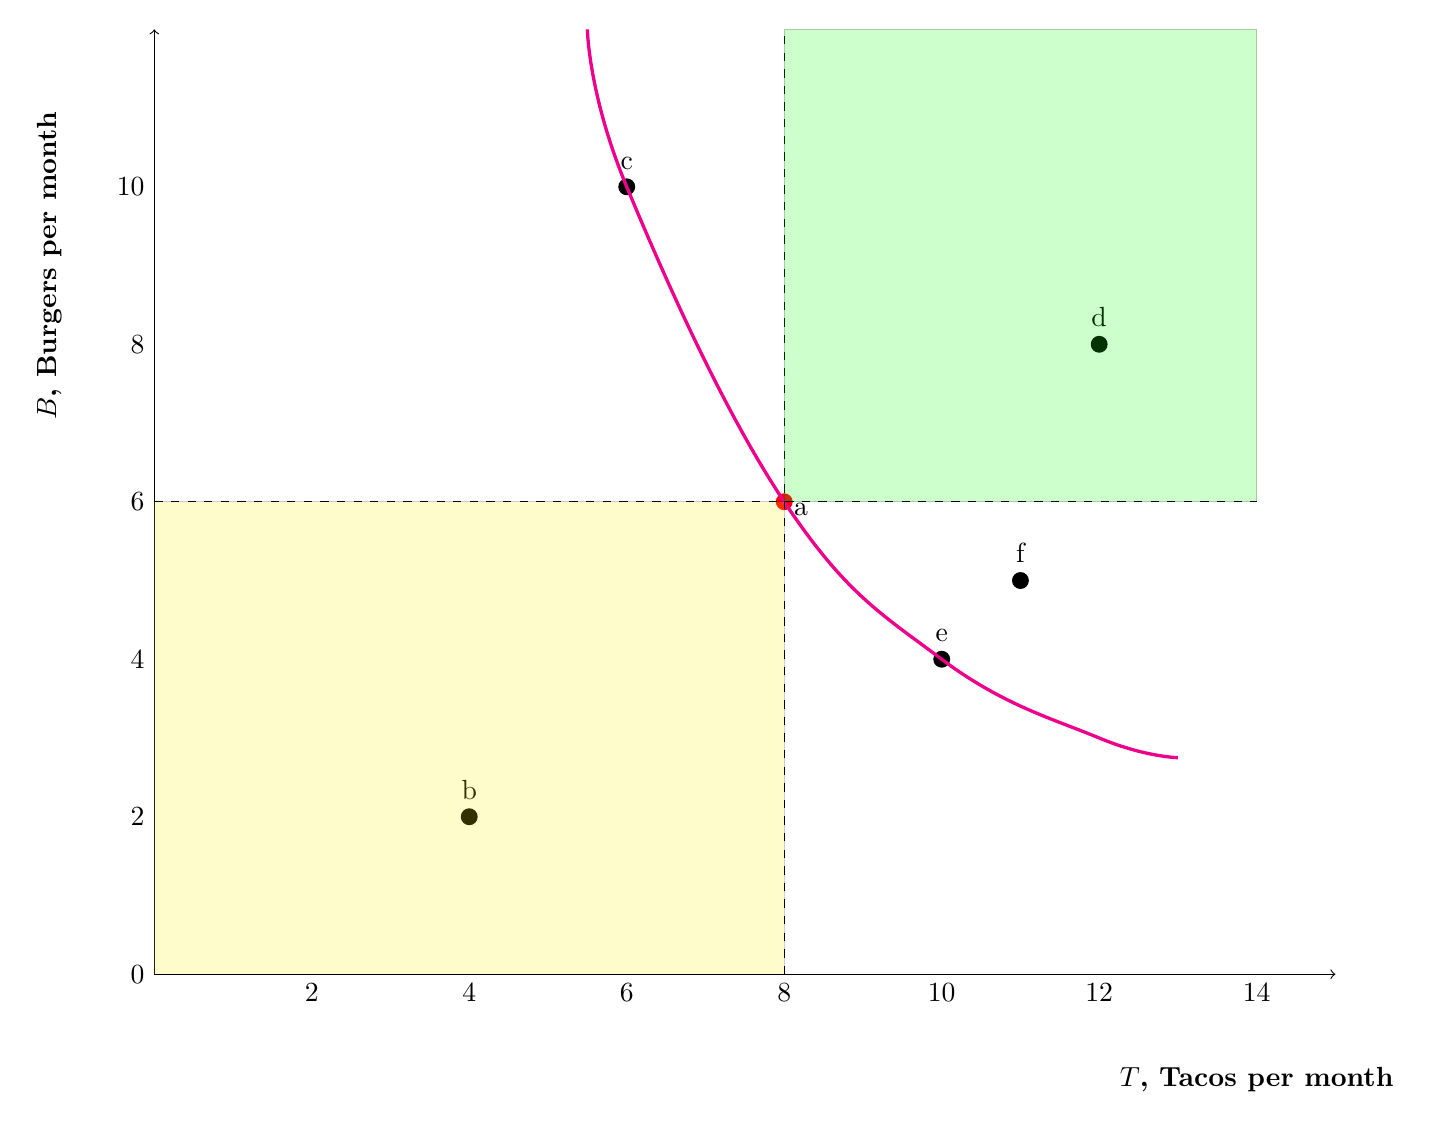
\begin{tikzpicture}
	% Draw axes
	%Y
	\draw[->] (0,0) -- (0,12) ;
	\draw[] (0,8) -- node[rotate=90, above=30pt] {\textbf{$B$, Burgers per month}} (0,10);
	%X
	\draw[->] (0,0) -- (15,0);
	\draw[] (14,0) -- node[below=30pt] {\textbf{$T$, Tacos per month}} (14,0);

	%Plot possible consumption bundles:
	%a
	\draw[fill, red] (8,6) circle [radius =0.1];
	\node at (8,6.1) [below right] {{a}};
	%b
	\draw[fill] (4,2) circle [radius =0.1];
	\node at (4,2.1) [above] {{b}};	
	%c
	\draw[fill] (6,10) circle [radius =0.1];
	\node at (6,10.1) [above] {{c}};
	%d
	\draw[fill] (12,8) circle [radius =0.1];
	\node at (12,8.1) [above] {{d}};
	%e
	\draw[fill] (10,4) circle [radius =0.1];
	\node at (10,4.1) [above] {{e}};
	%5
	\draw[fill] (11,5) circle [radius =0.1];
	\node at (11,5.1) [above] {{f}};

	%Plot indifference curves
	\draw[very thick, magenta] plot[smooth, tension=.7] coordinates {(5.5,12) (6,10) (8,6) (10,4) (12,3) (13,2.75)};

	%Plot illustrative lines
	\draw[dashed] (8,0) -- (8,12);
	\draw[fill=green, opacity=0.2]  (8,6) -- (8,12) -- (14,12) -- (14,6) -- cycle;

	\draw[dashed] (0,6) -- (14,6);
	\draw[fill=yellow, opacity=0.2]  (0,6) -- (8,6) -- (8,0) -- (0,0) -- cycle;

	%Add axes labels
	%Origin%
	\node at (0,0) [left] {{0}};
	%Y Axis
	\node at (0,2) [left] {{2}};
	\node at (0,4) [left] {{4}};
	\node at (0,6) [left] {{6}};
	\node at (0,8) [left] {{8}};
	\node at (0,10) [left] {{10}};

	%X Axis
	\node at (2,0) [below] {{2}};
	\node at (4,0) [below] {{4}};
	\node at (6,0) [below] {{6}};
	\node at (8,0) [below] {{8}};
	\node at (10,0) [below] {{10}};
	\node at (12,0) [below] {{12}};
	\node at (14,0) [below] {{14}};


\end{tikzpicture}
}
\caption{Taylor's Possible Choices}
\end{figure}
}

\frame{
	\frametitle{The Theory of Consumer Choice: Preferences}
	\begin{itemize}
	\item On the figure, the set of choices that Taylor is indifferent between is known as a \textit{indifference curve}.
	\item[]
	\item An indifference curve depicts the set of all bundles of goods that a consumer views as being equally desirable.
	\item[]
	\item We can repeat exercise to ask Taylor about all sets of indifferent choices.
		\begin{itemize}
		\item Result is an indifference map; a set of indifference curves that describes sets of goods that are viewed as equally desirable.
		\end{itemize}
	\end{itemize}
}

\frame{
	\frametitle{The Theory of Consumer Choice: Preferences}
	
	\begin{figure}[t!]
	\center
	\resizebox{!}{.45\linewidth}{

	\begin{tikzpicture}
	% Draw axes
	%Y
	\draw[->] (0,0) -- (0,12) ;
	\draw[] (0,8) -- node[rotate=90, above=30pt] {\textbf{$B$, Burgers per month}} (0,10);
	%X
	\draw[->] (0,0) -- (15,0);
	\draw[] (14,0) -- node[below=30pt] {\textbf{$T$, Tacos per month}} (14,0);

	%Plot possible consumption bundles:
	%a
	\draw[fill, red] (8,6) circle [radius =0.1];
	\node at (8,6.1) [below right] {{a}};
	%b
	\draw[fill] (4,2) circle [radius =0.1];
	\node at (4,2.1) [above] {{b}};	
	%c
	\draw[fill] (6,10) circle [radius =0.1];
	\node at (6,10.1) [above] {{c}};
	%d
	\draw[fill] (12,8) circle [radius =0.1];
	\node at (12,8.1) [above] {{d}};
	%e
	\draw[fill] (10,4) circle [radius =0.1];
	\node at (10,4.1) [above] {{e}};
	%5
%	\draw[fill] (11,5) circle [radius =0.1];
%	\node at (11,5.1) [above] {{f}};

	%Plot indifference curves
	\draw[very thick, magenta] plot[smooth, tension=.7] coordinates {(5.5,12) (6,10) (8,6) (10,4) (12,3) (13,2.75)};
	\draw[very thick, magenta] plot[smooth, tension=.7] coordinates {(10,12) (10.75,10) (12,8) (13,7.25)};
	\draw[very thick, magenta] plot[smooth, tension=.7] coordinates {(1,10) (2,6) (4,2) (7,0.25)};


	%Plot illustrative lines
%	\draw[dashed] (8,0) -- (8,12);
%	\draw[fill=green, opacity=0.2]  (8,6) -- (8,12) -- (14,12) -- (14,6) -- cycle;

%	\draw[dashed] (0,6) -- (14,6);
%	\draw[fill=yellow, opacity=0.2]  (0,6) -- (8,6) -- (8,0) -- (0,0) -- cycle;

	%Add axes labels
	%Origin%
	\node at (0,0) [left] {{0}};
	%Y Axis
	\node at (0,2) [left] {{2}};
	\node at (0,4) [left] {{4}};
	\node at (0,6) [left] {{6}};
	\node at (0,8) [left] {{8}};
	\node at (0,10) [left] {{10}};

	%X Axis
	\node at (2,0) [below] {{2}};
	\node at (4,0) [below] {{4}};
	\node at (6,0) [below] {{6}};
	\node at (8,0) [below] {{8}};
	\node at (10,0) [below] {{10}};
	\node at (12,0) [below] {{12}};
	\node at (14,0) [below] {{14}};


\end{tikzpicture}
}
\caption{Taylor's Indifference Map}
\end{figure}
}

\frame{
	\frametitle{The Theory of Consumer Choice: Preferences}
	\begin{itemize}
	\item Indifference maps must satisfy the following four properties:
		\begin{enumerate}
		\item Bundles on indifference curves farther from the origin are preferred to those on indifference curves closer to the origin.
		\item[]
		\item An indifference curve goes through every possible bundle.
		\item[]
		\item Indifference curves cannot cross.
		\item[]
		\item Indifference curves slope downward.
		\end{enumerate}
	\end{itemize}
}

\frame{
	\frametitle{The Theory of Consumer Choice: Preferences}
	
	\begin{figure}[t!]
	\center
	\resizebox{!}{.45\linewidth}{

	\begin{tikzpicture}
	% Draw axes
	%Y
	\draw[->] (0,0) -- (0,12) ;
	\draw[] (0,8) -- node[rotate=90, above=30pt] {\textbf{$B$, Burgers per month}} (0,10);
	%X
	\draw[->] (0,0) -- (15,0);
	\draw[] (14,0) -- node[below=30pt] {\textbf{$T$, Tacos per month}} (14,0);

	%Plot possible consumption bundles:
	%a
	\draw[fill, red] (8,6) circle [radius =0.1];
	\node at (8,6.1) [above right] {{a}};
	%b
%	\draw[fill] (4,2) circle [radius =0.1];
%	\node at (4,2.1) [above] {{b}};	
	%c
%	\draw[fill] (6,10) circle [radius =0.1];
%	\node at (6,10.1) [above] {{c}};
	%d
%	\draw[fill] (12,8) circle [radius =0.1];
%	\node at (12,8.1) [above] {{d}};
	%e
	\draw[fill] (10,4) circle [radius =0.1];
	\node at (10,4.1) [above] {{e}};
	%f
	\draw[fill] (11,5) circle [radius =0.1];
	\node at (11,5.1) [above] {{f}};

	%Plot indifference curves
	\draw[very thick, magenta] plot[smooth, tension=.7] coordinates {(5.5,12) (6,10) (8,6) (10,4) (12,3) (13,2.75)};
	\draw[very thick, magenta] plot[smooth, tension=.7] coordinates {(3,10) (5,8) (8,6) (11,5) (13,4.5)};


	%Plot illustrative lines
%	\draw[dashed] (8,0) -- (8,12);
%	\draw[fill=green, opacity=0.2]  (8,6) -- (8,12) -- (14,12) -- (14,6) -- cycle;

%	\draw[dashed] (0,6) -- (14,6);
%	\draw[fill=yellow, opacity=0.2]  (0,6) -- (8,6) -- (8,0) -- (0,0) -- cycle;

	%Add axes labels
	%Origin%
	\node at (0,0) [left] {{0}};
	%Y Axis
%	\node at (0,2) [left] {{2}};

	%X Axis
%	\node at (2,0) [below] {{2}};


\end{tikzpicture}
}
\caption{Impossible indifference curves}
\end{figure}
}

\frame{
	\frametitle{The Theory of Consumer Choice: Preferences}
	
	\begin{figure}[t!]
	\center
	\resizebox{!}{.45\linewidth}{

	\begin{tikzpicture}
	% Draw axes
	%Y
	\draw[->] (0,0) -- (0,12) ;
	\draw[] (0,8) -- node[rotate=90, above=30pt] {\textbf{$B$, Burgers per month}} (0,10);
	%X
	\draw[->] (0,0) -- (15,0);
	\draw[] (14,0) -- node[below=30pt] {\textbf{$T$, Tacos per month}} (14,0);

	%Plot possible consumption bundles:
	%a
	\draw[fill, red] (8,6) circle [radius =0.1];
	\node at (8,6.1) [above left] {{a}};
	%b
	\draw[fill] (4,2) circle [radius =0.1];
	\node at (4,2.1) [above] {{b}};	
	%c
%	\draw[fill] (6,10) circle [radius =0.1];
%	\node at (6,10.1) [above] {{c}};
	%d
%	\draw[fill] (12,8) circle [radius =0.1];
%	\node at (12,8.1) [above] {{d}};
	%e
%	\draw[fill] (10,4) circle [radius =0.1];
%	\node at (10,4.1) [above] {{e}};
	%f
%	\draw[fill] (11,5) circle [radius =0.1];
%	\node at (11,5.1) [above] {{f}};

	%Plot indifference curves
	\draw[very thick, magenta] plot[smooth, tension=.7] coordinates {(1,1) (4,2) (8,6) (10,11) };

	%Plot illustrative lines
%	\draw[dashed] (8,0) -- (8,12);
%	\draw[fill=green, opacity=0.2]  (8,6) -- (8,12) -- (14,12) -- (14,6) -- cycle;

%	\draw[dashed] (0,6) -- (14,6);
%	\draw[fill=yellow, opacity=0.2]  (0,6) -- (8,6) -- (8,0) -- (0,0) -- cycle;

	%Add axes labels
	%Origin%
	\node at (0,0) [left] {{0}};
	%Y Axis
%	\node at (0,2) [left] {{2}};

	%X Axis
%	\node at (2,0) [below] {{2}};


\end{tikzpicture}
}
\caption{An impossible indifference curve}
\end{figure}
}

\frame{
	\frametitle{The Theory of Consumer Choice: Preferences}
	\begin{itemize}
	\item Indifference curves contain a lot of information.
	\item[]
	\item The slope of the indifference curve reflects how willing consumers are to trade one good for another.
		\begin{itemize}
		\item This is known as the \textit{marginal rate of substitution}
		\end{itemize}
	\end{itemize}
	\begin{definition}[Marginal Rate of Substitution]
	The rate at which a consumer is willing to substitute one good for another.
	\end{definition}
	\begin{itemize}
	\item In our example, Taylor's marginal rate of substitution (MRS) is
		\begin{align*}
		MRS = \frac{\Delta B}{\Delta T}
		\end{align*}
	\end{itemize}
}

\frame{
	\frametitle{The Theory of Consumer Choice: Preferences}
	\begin{itemize}
	\item The curvature of the indifference curve also contains useful information.
		\begin{itemize}
		\item Curvature tells us how a consumer's willingness to substitute between goods changes as the relative quantity of each good changes.
		\end{itemize}
	\item[]
	\item If an indifference curve is convex (``bowed in'' towards the origin), preferences exhibit a \textit{diminishing marginal rate of substitution}.
	\item[]
	\item If an indifference curve is concave (``bowed out'' from the origin), preferences exhibit an \textit{increasing marginal rate of substitution}.
	\end{itemize}
}

\frame{
	\frametitle{The Theory of Consumer Choice: Preferences}
		
	\begin{figure}[t!]
	\center
	\resizebox{!}{.45\linewidth}{

	\begin{tikzpicture}
	% Draw axes
	%Y
	\draw[->] (0,0) -- (0,12) ;
	\draw[] (0,8) -- node[rotate=90, above=30pt] {\textbf{$B$, Burgers per month}} (0,10);
	%X
	\draw[->] (0,0) -- (15,0);
	\draw[] (14,0) -- node[below=30pt] {\textbf{$T$, Tacos per month}} (14,0);

	%Plot possible consumption bundles:
	%a
	\draw[fill] (2,8) circle [radius =0.1];
	\node at (2,8.1) [above] {{a}};
	%b
	\draw[fill] (4,5) circle [radius =0.1];
	\node at (4,5.1) [above] {{b}};	
	%c
	\draw[fill] (6,3) circle [radius =0.1];
	\node at (6,3.1) [above] {{c}};
	%d
	\draw[fill] (8,2) circle [radius =0.1];
	\node at (8,2.1) [above] {{d}};
	%e
%	\draw[fill] (10,1) circle [radius =0.1];
%	\node at (10,4.1) [above] {{e}};
	%f
%	\draw[fill] (11,5) circle [radius =0.1];
%	\node at (11,5.1) [above] {{f}};

	%Plot indifference curves
	\draw[very thick, magenta] plot[smooth, tension=.7] coordinates {(1,10) (2,8) (4,5) (6,3) (8,2) (10,1.5) };

	%Plot illustrative lines
	\draw[dashed] (2,8) -- (2,5) -- (4,5);
	\node at (2,6.5) [left] {{$\Delta B = -3$}};
	\node at (3,5) [above] {{$\Delta T = 2$}};
	
	\draw[dashed] (4,5) -- (4,3) -- (6,3);
	\node at (4,4) [left] {{$\Delta B = -2$}};
	\node at (5,3) [above] {{$\Delta T = 2$}};
	
	\draw[dashed] (6,3) -- (6,2) -- (8,2);
	\node at (6,2.5) [left] {{$\Delta B = -1$}};
	\node at (7,2) [below] {{$\Delta T = 2$}};
	
	%Add axes labels
	%Origin%
	\node at (0,0) [left] {{0}};
	%Y Axis
	\node at (0,2) [left] {{2}};
	\node at (0,3) [left] {{3}};
	\node at (0,5) [left] {{5}};
	\node at (0,8) [left] {{8}};

	%X Axis
	\node at (2,0) [below] {{2}};
	\node at (4,0) [below] {{4}};
	\node at (6,0) [below] {{6}};
	\node at (8,0) [below] {{8}};

\end{tikzpicture}
}
\caption{Convex Preferences}
\end{figure}
}

\frame{
	\frametitle{The Theory of Consumer Choice: Preferences}
		
	\begin{figure}[t!]
	\center
	\resizebox{!}{.45\linewidth}{

	\begin{tikzpicture}
	% Draw axes
	%Y
	\draw[->] (0,0) -- (0,12) ;
	\draw[] (0,8) -- node[rotate=90, above=30pt] {\textbf{$B$, Burgers per month}} (0,10);
	%X
	\draw[->] (0,0) -- (15,0);
	\draw[] (14,0) -- node[below=30pt] {\textbf{$T$, Tacos per month}} (14,0);

	%Plot possible consumption bundles:
	%a
	\draw[fill] (2,8) circle [radius =0.1];
	\node at (2,8.1) [above] {{a}};
	%b
	\draw[fill] (4,7) circle [radius =0.1];
	\node at (4,7.1) [above] {{b}};	
	%c
	\draw[fill] (6,5) circle [radius =0.1];
	\node at (6,5.1) [above] {{c}};
	%d
	\draw[fill] (8,2) circle [radius =0.1];
	\node at (8,2.1) [above] {{d}};
	%e
%	\draw[fill] (10,1) circle [radius =0.1];
%	\node at (10,4.1) [above] {{e}};
	%f
%	\draw[fill] (11,5) circle [radius =0.1];
%	\node at (11,5.1) [above] {{f}};

	%Plot indifference curves
	\draw[very thick, magenta] plot[smooth, tension=.7] coordinates {(0.5,8.5) (2,8) (4,7) (6,5) (8,2) (8.5,.5) };

	%Plot illustrative lines
	\draw[dashed] (2,8) -- (2,7) -- (4,7);
	\node at (2,7.5) [left] {{$\Delta B = -1$}};
	\node at (3,7) [below] {{$\Delta T = 2$}};
	
	\draw[dashed] (4,7) -- (4,5) -- (6,5);
	\node at (4,6) [left] {{$\Delta B = -2$}};
	\node at (5,5) [below] {{$\Delta T = 2$}};
	
	\draw[dashed] (6,5) -- (6,2) -- (8,2);
	\node at (6,3.5) [left] {{$\Delta B = -3$}};
	\node at (7,2) [below] {{$\Delta T = 2$}};
	
	%Add axes labels
	%Origin%
	\node at (0,0) [left] {{0}};
	%Y Axis
	\node at (0,2) [left] {{2}};
	\node at (0,3) [left] {{3}};
	\node at (0,5) [left] {{5}};
	\node at (0,8) [left] {{8}};

	%X Axis
	\node at (2,0) [below] {{2}};
	\node at (4,0) [below] {{4}};
	\node at (6,0) [below] {{6}};
	\node at (8,0) [below] {{8}};

\end{tikzpicture}
}
\caption{Concave Preferences}
\end{figure}
}

\frame{
	\frametitle{The Theory of Consumer Choice: Preferences}
	\begin{itemize}
	\item Empirical evidence suggests that most people have convex indifference curves for most pairs of products.
	\item[]
	\item In one extreme case, preferences exhibit a constant marginal rate of substitution, meaning goods are \textit{perfect substitutes}.
		\begin{itemize}
		\item Perfect substitutes are goods that are essentially equivalent from the consumer's point of view.
		\end{itemize}
	\item[]
	\item At the other extreme, goods are always consumed in fixed proportions.
		\begin{itemize}
		\item In this case, goods are known as \textit{perfect complements}.
		\end{itemize}
	\end{itemize}
}

\frame{
	\frametitle{The Theory of Consumer Choice: Preferences}
		
	\begin{figure}[t!]
	\center
	\resizebox{!}{.45\linewidth}{

	\begin{tikzpicture}
	% Draw axes
	%Y
	\draw[->] (0,0) -- (0,13) ;
	\draw[] (0,8) -- node[rotate=90, above=30pt] {Coke, Cans per day} (0,10);
	%X
	\draw[->] (0,0) -- (15,0);
	\draw[] (14,0) -- node[below=30pt] {Pepsi, Cans per day} (14,0);

	%Plot Indifference Curves
	\draw[very thick, magenta] plot[smooth, tension=.7] coordinates {(0,3) (3,0)};
	\draw[very thick, magenta] plot[smooth, tension=.7] coordinates {(0,6) (6,0)};
	\draw[very thick, magenta] plot[smooth, tension=.7] coordinates {(0,9) (9,0)};
	\draw[very thick, magenta] plot[smooth, tension=.7] coordinates {(0,12) (12,0)};
	
	%Add axes labels
	%Origin%
	\node at (0,0) [left] {{0}};
	%Y Axis
	\node at (0,3) [left] {{1}};
	\node at (0,6) [left] {{2}};
	\node at (0,9) [left] {{3}};
	\node at (0,12) [left] {{4}};

	%X Axis
	\node at (3,0) [below] {{1}};
	\node at (6,0) [below] {{2}};
	\node at (9,0) [below] {{3}};
	\node at (12,0) [below] {{4}};

\end{tikzpicture}
}
\caption{Perfect substitutes}
\end{figure}
}

\frame{
	\frametitle{The Theory of Consumer Choice: Preferences}
		
	\begin{figure}[t!]
	\center
	\resizebox{!}{.45\linewidth}{

	\begin{tikzpicture}
	% Draw axes
	%Y
	\draw[->] (0,0) -- (0,13) ;
	\draw[] (0,8) -- node[rotate=90, above=30pt] {Ice Cream, Scoops per day} (0,10);
	%X
	\draw[->] (0,0) -- (15,0);
	\draw[] (14,0) -- node[below=30pt] {Pie, Pieces per day} (14,0);

	%Plot Indifference Curves
	\draw[very thick, magenta] (3,12) -- (3,3) -- (12,3) ;
	\draw[fill] (3,3) circle [radius =0.1];
	\node at (3,3.1) [above right] {{a}};
	\draw[fill] (3,6) circle [radius =0.1];
	\node at (3,6.1) [above right] {{d}};
	\draw[fill] (3,9) circle [radius =0.1];
	\node at (3,9.1) [above right] {{e}};
	\draw[very thick, magenta] (6,12) -- (6,6) -- (12,6) ;
	\draw[fill] (6,6) circle [radius =0.1];
	\node at (6,6.1) [above right] {{b}};
	\draw[very thick, magenta] (9,12) -- (9,9) -- (12,9) ;
	\draw[fill] (9,9) circle [radius =0.1];
	\node at (9,9.1) [above right] {{c}};
	
	%Add axes labels
	%Origin%
	\node at (0,0) [left] {{0}};
	%Y Axis
	\node at (0,3) [left] {{1}};
	\node at (0,6) [left] {{2}};
	\node at (0,9) [left] {{3}};
	\node at (0,12) [left] {{4}};

	%X Axis
	\node at (3,0) [below] {{1}};
	\node at (6,0) [below] {{2}};
	\node at (9,0) [below] {{3}};
	\node at (12,0) [below] {{4}};

\end{tikzpicture}
}
\caption{Perfect Compliments}
\end{figure}
}

\frame{
	\frametitle{The Theory of Consumer Choice: Preferences}
	\begin{itemize}
	\item Typically, preferences lie between the two extremes, meaning that goods are \textit{imperfect substitutes}.
	\end{itemize}
}

\frame{
	\frametitle{The Theory of Consumer Choice: Preferences}
		
	\begin{figure}[t!]
	\center
	\resizebox{!}{.45\linewidth}{

	\begin{tikzpicture}
	% Draw axes
	%Y
	\draw[->] (0,0) -- (0,12) ;
	\draw[] (0,8) -- node[rotate=90, above=30pt] {\textbf{$B$, Burgers per month}} (0,10);
	%X
	\draw[->] (0,0) -- (15,0);
	\draw[] (14,0) -- node[below=30pt] {\textbf{$T$, Tacos per month}} (14,0);

	%Plot Indifference Curves
	\draw[very thick, magenta] plot[smooth, tension=.7] coordinates {(2,10) (4,4) (10,2) };
	\draw[dashed, magenta] (0,8) -- (8,0) ;
	\draw[dashed, magenta] (4,12) -- (4,4) -- (12,4) ;

	%Add axes labels
	%Origin%
	\node at (0,0) [left] {{0}};
	%Y Axis
%	\node at (0,3) [left] {{1}};
%	\node at (0,6) [left] {{2}};
%	\node at (0,9) [left] {{3}};
%	\node at (0,12) [left] {{4}};

	%X Axis
%	\node at (3,0) [below] {{1}};
%	\node at (6,0) [below] {{2}};
%	\node at (9,0) [below] {{3}};
%	\node at (12,0) [below] {{4}};

\end{tikzpicture}
}
\caption{Imperfect Substitutes}
\end{figure}
}

\frame{
	\frametitle{The Theory of Consumer Choice: Utility}
	\begin{itemize}
	\item Our model of consumer behaviour assumes that consumers can compare bundles of goods and services to decide which gives them the greatest satisfaction.
	\item[]
	\item We can summarize these preferences by giving each bundle of goods and services that can be consumed a numerical value that reflects the relative ranking of the bundles.
	\item[]
	\item These numeric values describe the \textit{utility} from consumption.
	\item[]
	\item The idea of describing preferences with utility is quite old.
		\begin{itemize}
		\item Goes back to the 19th century and the work of John Stuart Mill and Jeremy Bentham.
		\end{itemize}
	\end{itemize}
}

\frame{
	\frametitle{The Theory of Consumer Choice: Utility}
	\begin{itemize}
	\item The idea of utility is quite powerful because it lets us summarize the information contained in an indifference map succinctly using a \textit{utility function}.
	\item[]
	\item The utility function describes the level of utility obtained from consuming goods and services:
		\begin{align*}
		U = U(B,T)
		\end{align*}
	where $U$ is the level of utility obtained from consuming $B$ and $T$ respectively.
	\item[]
	\item Given a utility function, $U(-)$, if a consumer prefers bundle $(B_{1},T_{1})$ to bundle $(B_{2},T_{2})$, then $U(B_{1},T_{1})>U(B_{2},T_{2})$.
	\end{itemize}
}

\frame{
	\frametitle{The Theory of Consumer Choice: Utility Example}
	\begin{itemize}
	\item Suppose Taylor's utility function for burgers and tacos is given by:
		\begin{align*}
		U = \sqrt{(B \times T)}
		\end{align*}
	and suppose Taylor faces a choice between consuming 4 burgers and 25 tacos, or 9 burgers and 9 tacos.
	\item Then the utility Taylor receives from consuming 4 burgers and 25 tacos is 10 ($=\sqrt{(4 \times 25)}$).
	\item And the utility Taylor receives from consuming 9 burgers and 9 tacos is 9 ($=\sqrt{(9 \times 9)}$).
	\item Thus, Taylor prefers the first bundle of goods.
	\end{itemize}
}

\frame{
	\frametitle{The Theory of Consumer Choice: 2 Points about Utility}
	\begin{enumerate}
	\item Utility functions do not exist in any fundamental sense.
	\item[]
	\item Utility is an \textit{ordinal} measure.
		\begin{itemize}
		\item An ordinal measure only contains information about relative rankings.
			\begin{itemize}
			\item E.g. 5 star vs 1 star Google review.
			\end{itemize}
		\item Cardinal measures are based on absolute numerical comparisons.
			\begin{itemize}
			\item E.g. 10 kg vs 20 kg.
			\end{itemize}
		\end{itemize}
	\end{enumerate}
}

\frame{
	\frametitle{The Theory of Consumer Choice: Utility}
	\begin{itemize}
	\item We can use the utility function to understand how preferences change as consumption bundles change.
	\item[]
	\item The extra utility ($\Delta U$) that a consumer gets from consuming an additional unit of a good (e.g. $\Delta B = 1$ or $\Delta T = 1$) is the \textit{marginal utility} from that good.
	\item[]
	\item Marginal utility (MU) tells us how utility changes as we increase (or decrease) consumption of one good, holding consumption of all other goods constant.
		\begin{itemize}
		\item It is the \textit{slope} of the utility function holding consumption of other goods constant:
			\begin{align*}
			MU_{B} = \Delta U/\Delta B
			\end{align*}
		\end{itemize}
	\end{itemize}	
}

\frame{
	\frametitle{The Theory of Consumer Choice: Marginal Utility}
	\begin{itemize}
	\item As an example, again suppose Taylor's utility function is given by $U=\sqrt{B \times T}$, and suppose that Taylor consumes 10 burgers.
	\item[]
	\item What happens to Taylor's utility and marginal utility is they consume 6 tacos instead of 7?
	\end{itemize}
}

\frame{
	\frametitle{The Theory of Consumer Choice: Marginal Utility}
		
	\begin{figure}[t!]
	\center
	\resizebox{!}{.45\linewidth}{

	\begin{tikzpicture}
	% Draw axes
	%Y
	\draw[->] (0,0) -- (0,12) ;
	\draw[] (0,8) -- node[rotate=90, above=30pt] {\textbf{$U$, Utils}} (0,10);
	%X
	\draw[->] (0,0) -- (15,0);
	\draw[] (14,0) -- node[below=30pt] {\textbf{$T$, Tacos per month}} (14,0);

	%Plot  Curves
	\draw[color=black, very thick, domain=0:12] plot (\x,{sqrt(10*\x)});
	\node at (12,11) [right] {{Utility function, $U(10,T)$}};

	\draw[dashed] (0,7.75) -- (6,7.75) -- (6,0);
	\draw[dashed] (0,8.36) -- (7,8.36) -- (7,0);
	\draw[dashed] (6,7.75) -- (7,7.75);
	
	\node at (7,8) [right] {{$\Delta U = 0.61$}};
	\node at (6.5,7.75) [below] {{$\Delta T = 1$}};
	
	%Add axes labels
	%Origin%
	\node at (0,0) [left] {{0}};
	%Y Axis
	\node at (0,7.75) [left] {{7.75}};
	\node at (0,8.36) [left] {{8.36}};

	%X Axis
	\node at (1,0) [below] {{1}};
	\node at (2,0) [below] {{2}};
	\node at (3,0) [below] {{3}};
	\node at (4,0) [below] {{4}};
	\node at (5,0) [below] {{5}};
	\node at (6,0) [below] {{6}};
	\node at (7,0) [below] {{7}};
	\node at (8,0) [below] {{8}};
	\node at (9,0) [below] {{9}};
	\node at (10,0) [below] {{10}};
	\node at (11,0) [below] {{11}};
	\node at (12,0) [below] {{12}};

\end{tikzpicture}
}
\caption{The effect of a one taco increase}
\end{figure}
}

\frame{
	\frametitle{The Theory of Consumer Choice: Utility}
	\begin{itemize}
	\item Recall: The marginal rate of substitution tells us the rate at which a consumer is willing to substitute one good for another.
	\item[]
	\item Given that marginal utility tells us how much consumer satisfaction changes if consumption changes by one unit, we can re-express MRS in terms of marginal utility.
		\begin{align*}
		MRS = \frac{\Delta B}{\Delta T} = - \frac{MU_{T}}{MU_{B}}
		\end{align*}
	\end{itemize}
}

\frame{
	\frametitle{The Theory of Consumer Choice: An Application of Utility}
	\begin{itemize}
	\item The idea that we can understand consumer choice by exploiting utility functions has been quite powerful in practice.
	\item[]
	\item A good example of this is the work of Dan McFadden (Nobel Prize, 2000) examining the potential usage of the Bay Area Rapid Transit (BART) system in the early 1970s.
	\end{itemize}
}

\frame{
	\frametitle{The Theory of Consumer Choice: An Application of Utility}
	\begin{itemize}
	\item McFadden and his research team collected data on the travel behaviour of several hundred individuals in the San Francisco Bay Area in 1972, prior to BART's introduction.
	\item[]
	\item They applied the theory of consumer choice to predict what the travel behaviour of these individuals would be in 1975, after BART's introduction.
	\item[]
	\item The data suggests the theory did a good job of predicting consumer behaviour.
	\end{itemize}
}

\frame{
	\frametitle{The Theory of Consumer Choice: An Application of Utility}
	\begin{figure}
	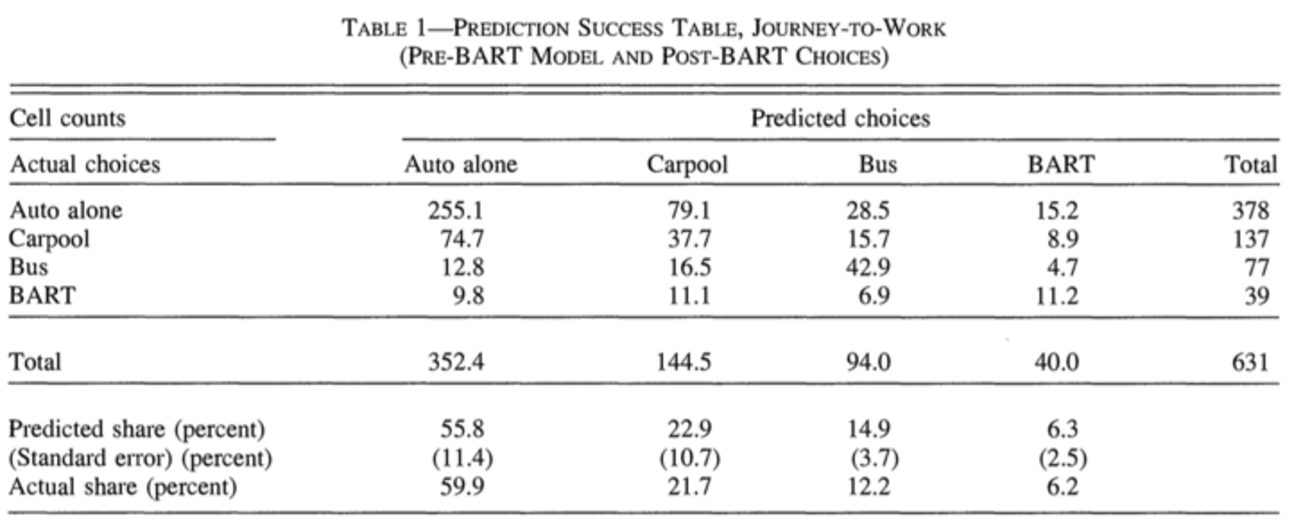
\includegraphics[scale=0.6]{../images/bart.pdf}
	\end{figure}

}

\frame{
	\frametitle{The Theory of Consumer Choice: The Budget Constraint}
	\begin{itemize}
	\item Understanding preferences is the first step in determining consumer choice behaviour.
	\item[]
	\item The second step is understanding the constraints consumers face when making decisions.
	\item[]
	\item The most important constraint individuals face in the standard theory of consumer choice is the limitations imposed by a budget.
	\end{itemize}
}

\frame{
	\frametitle{The Theory of Consumer Choice: The Budget Constraint}
	\begin{itemize}
	\item For simplicity, let's again consider the case of Taylor, who spends all of their money on burgers and tacos. Taylor's budget constraint is then:
		\begin{align*}
		p_{B} B + p_{T} T = Y
		\end{align*}
	where $p_{B}$ is the price of burgers, $p_{T}$ is the price of tacos, and $Y$ is income.
	\item[]
	\item We can re-express Taylor's budget constraint in terms of $B$:
		\begin{align*}
		B = \frac{Y}{p_{B}} - \frac{p_{T}}{p_{B}} T
		\end{align*}
	\end{itemize}
}

\frame{
	\frametitle{The Theory of Consumer Choice: The Budget Constraint}
		
	\begin{figure}[t!]
	\center
	\resizebox{!}{.45\linewidth}{

	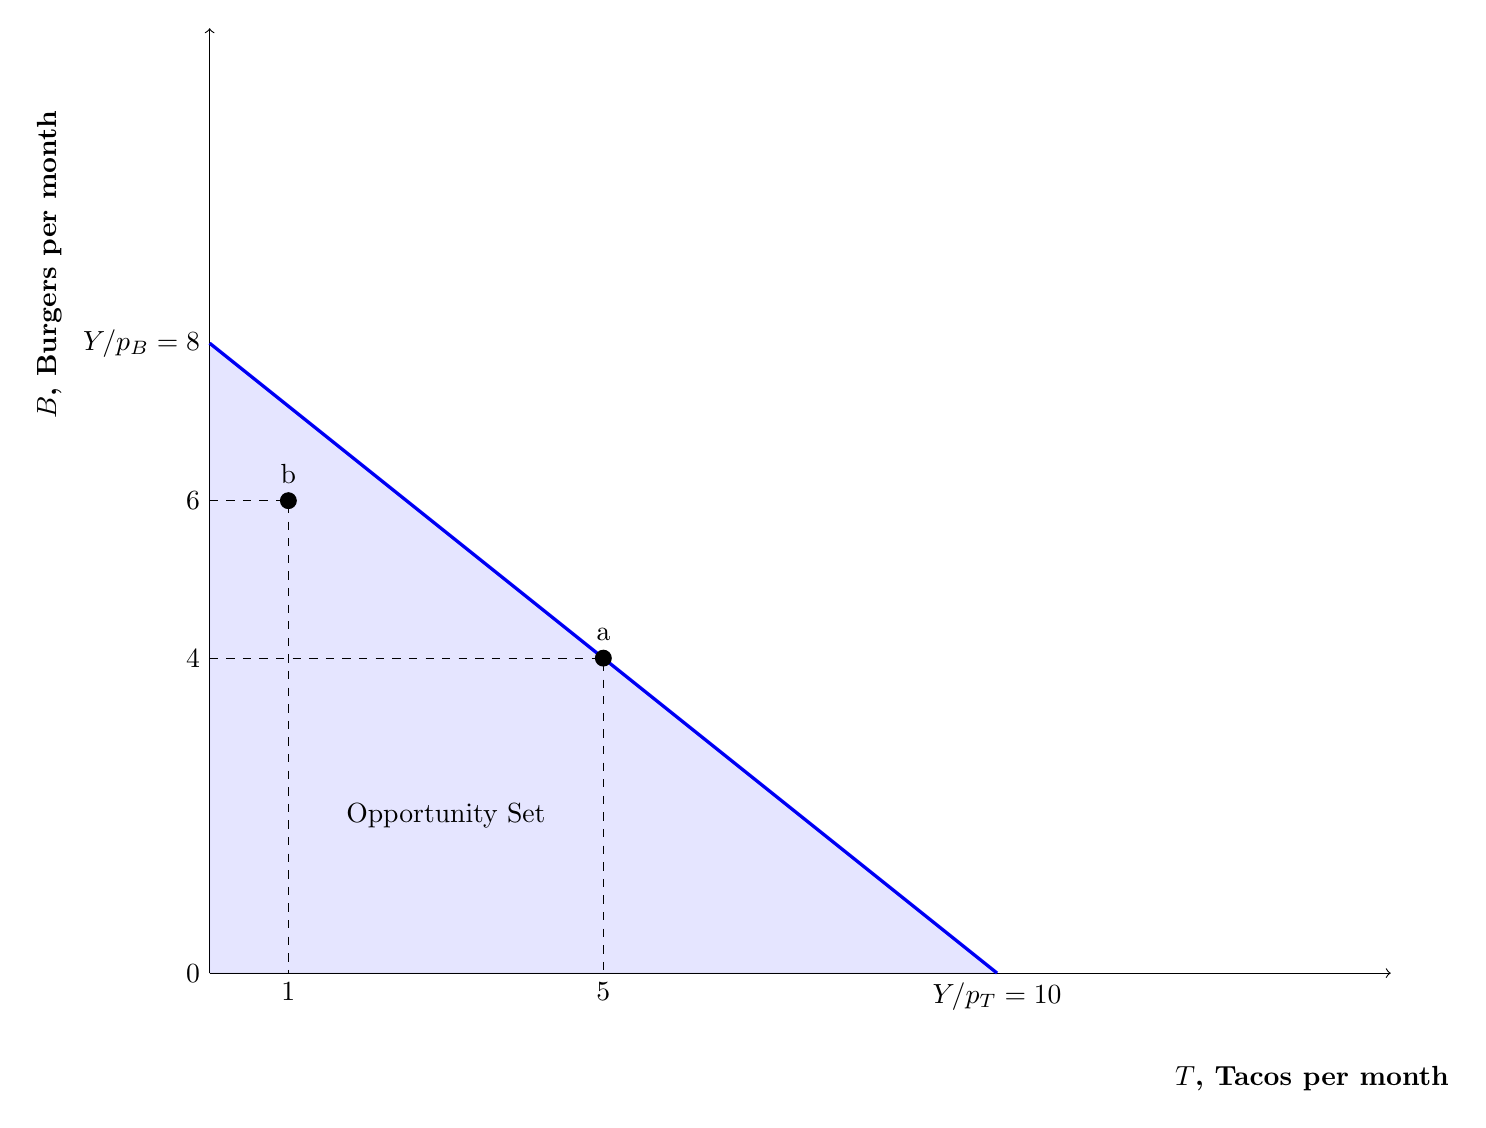
\begin{tikzpicture}
	% Draw axes
	%Y
	\draw[->] (0,0) -- (0,12) ;
	\draw[] (0,8) -- node[rotate=90, above=50pt] {\textbf{$B$, Burgers per month}} (0,10);
	%X
	\draw[->] (0,0) -- (15,0);
	\draw[] (14,0) -- node[below=30pt] {\textbf{$T$, Tacos per month}} (14,0);

	%Plot Budget Constraint
	% Y=40
	% p_T=4
	% p_B=5
	\draw[color=blue, very thick, domain=0:10] plot (\x,{(40/5)-(4/5)*\x});
	\draw[fill=blue, opacity=0.1]  (0,8) -- (0,0) -- (10,0)  -- cycle;
	\node at (3,2) {{Opportunity Set}};

	\draw[dashed] (0,4) -- (5,4) -- (5,0);
	\draw[fill] (5,4) circle [radius =0.1];
	\node at (5,4.1) [above] {{a}};

	\draw[dashed] (0,6) -- (1,6) -- (1,0);
	\draw[fill] (1,6) circle [radius =0.1];
	\node at (1,6.1) [above] {{b}};

	%Add axes labels
	%Origin%
	\node at (0,0) [left] {{0}};
	%Y Axis
	\node at (0,8) [left] {{$Y/p_{B}=8$}};
	\node at (0,4) [left] {{$4$}};
	\node at (0,6) [left] {{$6$}};

	%X Axis
	\node at (10,0) [below] {{$Y/p_{T}=10$}};
	\node at (5,0) [below] {{$5$}};
	\node at (1,0) [below] {{$1$}};

\end{tikzpicture}
}
\caption{Budget constraint with $Y=40$, $p_{B}=5$, and $p_{T}=4$.}
\end{figure}
}

\frame{
	\frametitle{The Theory of Consumer Choice: The Budget Constraint}
	\begin{itemize}
	\item The \textit{budget constraint} or \textit{budget line} depicts all possible bundles of goods that can be purchased if the consumer's entire budget is spent on those goods at given prices.
	\item[]
	\item The \textit{opportunity set} is the set of all possible bundles of goods that a consumer can buy.
	\end{itemize}
}

\frame{
	\frametitle{The Theory of Consumer Choice: The Budget Constraint}
	\begin{itemize}
	\item The budget constraint contains useful information.
	\item[]
	\item The slope of the budget constraint is known as the \textit{marginal rate of transformation} (MRT).
	\end{itemize}
	\begin{definition}[Marginal Rate of Transformation]
	The trade-off the market imposes on the consumer in terms of how much of one good the consumer must give up to purchase more of another good.
	\end{definition}
	\begin{itemize}
	\item In our example, the MRT is given by:
		\begin{align*}
		MRT = -\frac{p_{T}}{p_{B}}
		\end{align*}
	\end{itemize}
}

\frame{
	\frametitle{The Theory of Consumer Choice: The Budget Constraint}
	\begin{itemize}
	\item Changes in prices and income change the opportunity set.
	\item[]
	\item As an example, first consider the effect of a \$1 decrease in the price of tacos.
	\end{itemize}
}

\frame{
	\frametitle{The Theory of Consumer Choice: The Budget Constraint}
		
	\begin{figure}[t!]
	\center
	\resizebox{!}{.45\linewidth}{

	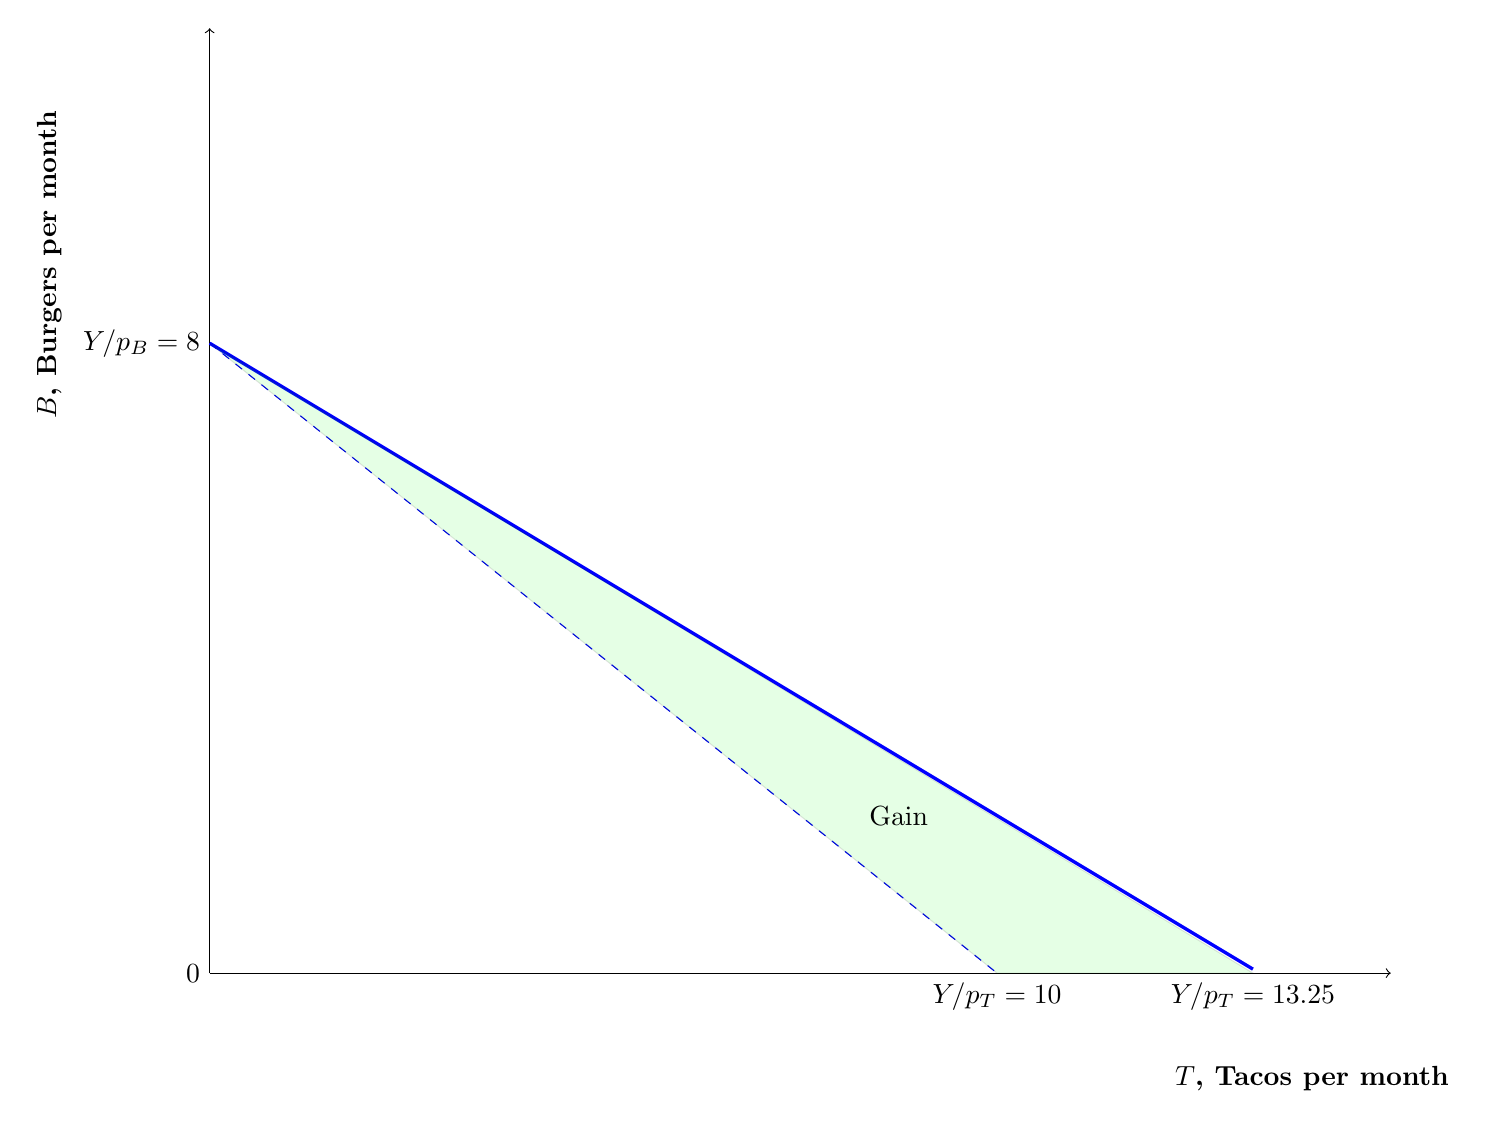
\begin{tikzpicture}
	% Draw axes
	%Y
	\draw[->] (0,0) -- (0,12) ;
	\draw[] (0,8) -- node[rotate=90, above=50pt] {\textbf{$B$, Burgers per month}} (0,10);
	%X
	\draw[->] (0,0) -- (15,0);
	\draw[] (14,0) -- node[below=30pt] {\textbf{$T$, Tacos per month}} (14,0);

	%Plot Budget Constraint
	% Y=40
	% p_T=4
	% p_B=5
	\draw[color=blue, dashed, domain=0:10] plot (\x,{(40/5)-(4/5)*\x});
	\draw[color=blue, very thick, domain=0:13.25] plot (\x,{(40/5)-(3/5)*\x});
	
	\draw[fill=green, opacity=0.1]  (0,8) -- (10,0) -- (13.25,0)  -- cycle;
	\node at (8.75,2) {{Gain}};

	%Add axes labels
	%Origin%
	\node at (0,0) [left] {{0}};
	%Y Axis
	\node at (0,8) [left] {{$Y/p_{B}=8$}};

	%X Axis
	\node at (10,0) [below] {{$Y/p_{T}=10$}};
	\node at (13.25,0) [below] {{$Y/p_{T}=13.25$}};

\end{tikzpicture}
}
\caption{The effect of a \$1 decrease in the price of tacos.}
\end{figure}
}

\frame{
	\frametitle{The Theory of Consumer Choice: The Budget Constraint}
	\begin{itemize}
	\item Next,  consider the effect of a \$20 decrease in income.
	\end{itemize}
}

\frame{
	\frametitle{The Theory of Consumer Choice: The Budget Constraint}
		
	\begin{figure}[t!]
	\center
	\resizebox{!}{.45\linewidth}{

	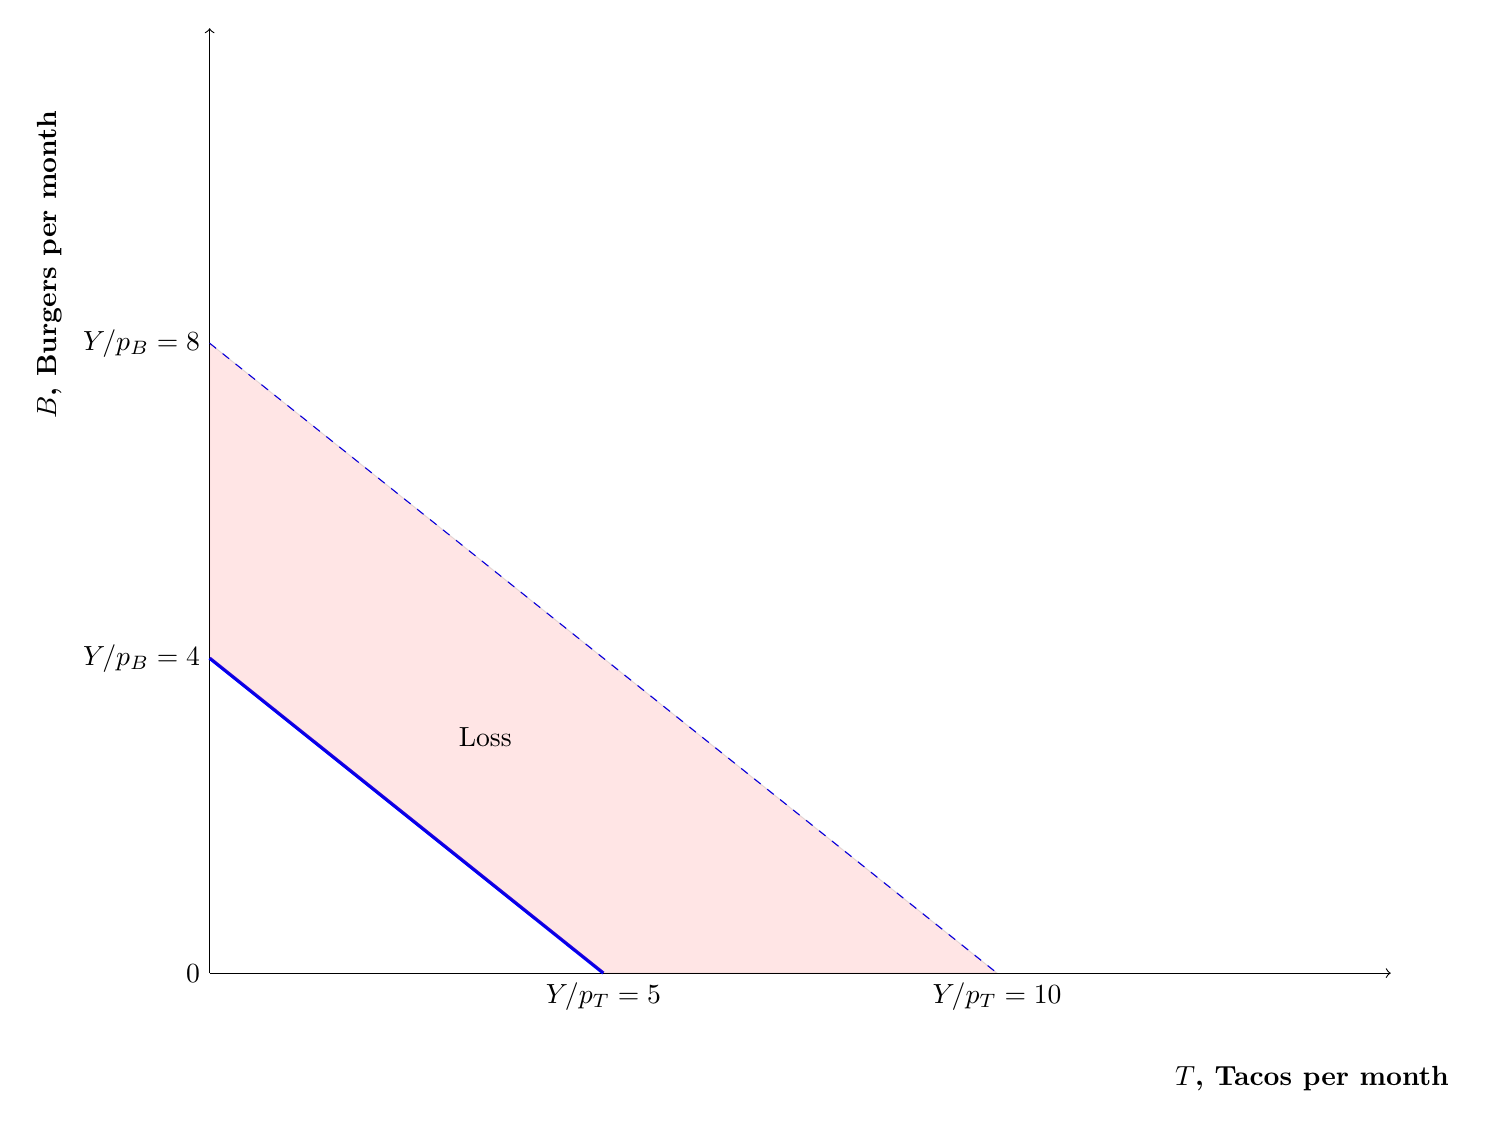
\begin{tikzpicture}
	% Draw axes
	%Y
	\draw[->] (0,0) -- (0,12) ;
	\draw[] (0,8) -- node[rotate=90, above=50pt] {\textbf{$B$, Burgers per month}} (0,10);
	%X
	\draw[->] (0,0) -- (15,0);
	\draw[] (14,0) -- node[below=30pt] {\textbf{$T$, Tacos per month}} (14,0);

	%Plot Budget Constraint
	% Y=40
	% p_T=4
	% p_B=5
	\draw[color=blue, dashed, domain=0:10] plot (\x,{(40/5)-(4/5)*\x});
	\draw[color=blue, very thick, domain=0:5] plot (\x,{(20/5)-(4/5)*\x});
	\draw[fill=red, opacity=0.1]  (0,8) -- (0,4) -- (5,0) -- (10,0) -- cycle;
	\node at (3.5,3) {{Loss}};

	%Add axes labels
	%Origin%
	\node at (0,0) [left] {{0}};
	%Y Axis
	\node at (0,8) [left] {{$Y/p_{B}=8$}};
	\node at (0,4) [left] {{$Y/p_{B}=4$}};
	%X Axis
	\node at (10,0) [below] {{$Y/p_{T}=10$}};
	\node at (5,0) [below] {{$Y/p_{T}=5$}};


\end{tikzpicture}
}
\caption{The effects of a \$20 income decrease.}
\end{figure}
}

\frame{
	\frametitle{The Theory of Consumer Choice: Determining Choice}
	\begin{itemize}
	\item The third step in determining consumer choice behaviour is understanding how consumers maximize their well-being, subject to the constraints that they face.
	\item[]
	\item Basic idea underlying our theory: Constrained consumer choice.
		\begin{itemize}
		\item Consumers pick the bundle of goods in their opportunity set that gives them the highest level of utility.
		\item Intuition: of all the bundles of goods that they can afford to buy, consumers choose the bundle of goods that makes them the happiest.
		\end{itemize}
	\end{itemize}
}

\frame{
	\frametitle{The Theory of Consumer Choice: Constrained Consumer Choice}
	\begin{itemize}
	\item If consumers choose the bundle of goods that makes them the happiest, their optimal choice must lie on an indifference curve that touches the budget line, but does not cross it.
	\item[]
	\item Why is this?
	\end{itemize}
}

\frame{
	\frametitle{The Theory of Consumer Choice: Constrained Consumer Choice}
	\begin{itemize}
	\item There are two ways consumers can reach their optimal bundle:
		\begin{enumerate}
		\item An \textit{interior solution}, where the optimal bundle has positive quantities of all goods, and lies between the ends of the budget line.
		\item[]
		\item A \textit{corner solution}, where the optimal bundle has a quantity of zero for at least one good, meaning the optimal bundle is at one end of the budget line.
		\end{enumerate}
	\end{itemize}	
}

\frame{
	\frametitle{The Theory of Consumer Choice: Constrained Consumer Choice}

	\begin{figure}[t!]
	\center
	\resizebox{!}{.4\linewidth}{

	\begin{tikzpicture}
	% Draw axes
	%Y
	\draw[->] (0,0) -- (0,12) ;
	\draw[] (0,8) -- node[rotate=90, above=50pt] {\textbf{$B$, Burgers per month}} (0,10);
	%X
	\draw[->] (0,0) -- (15,0);
	\draw[] (14,0) -- node[below=30pt] {\textbf{$T$, Tacos per month}} (14,0);

	%Plot Budget Constraint
	% Y=40
	% p_T=4
	% p_B=5
	\draw[color=blue, very thick, domain=0:10] plot (\x,{(40/5)-(4/5)*\x});
	\draw[color=magenta, very thick, domain=2:12] plot (\x,{(20/\x)});
	
	\draw[dashed] (0,4) -- (5,4) -- (5,0);
	
	%Add axes labels
	%Origin%
	\node at (0,0) [left] {{0}};
	%Y Axis
	\node at (0,8) [left] {{$Y/p_{B}=8$}};
	\node at (0,4) [left] {{$4$}};
	%X Axis
	\node at (10,0) [below] {{$Y/p_{T}=10$}};
	\node at (5,0) [below] {{$5$}};


\end{tikzpicture}
}
\caption{An Interior Solution.}
\end{figure}

}

\frame{
	\frametitle{The Theory of Consumer Choice: Solving for an Interior Solution}
	\begin{itemize}
	\item At an interior solution, the consumer's indifference curve is \textit{tangent} to the budget line.
		\begin{itemize}
		\item This means that the slope of the budget line and slope of the indifference curve are equal.
		\end{itemize}
	\item[]
	\item This means that $MRS=MRT$ at an interior solution, so:
		\begin{align*}
		MRS = - \frac{MU_{T}}{MU_{B}} = - \frac{p_{T}}{p_{B}} = MRT
		\end{align*}
	or equivalently:
		\begin{align*}
		\frac{MU_{T}}{p_{T}} =  \frac{MU_{B}}{p_{B}}
		\end{align*}
	\end{itemize}
}

\frame{
	\frametitle{The Theory of Consumer Choice: An Interior Example}
	\begin{itemize}
	\item Suppose Nate's utility function over strawberry jelly, $J$, and peanut butter, $N$, is $U=NJ$. As such, Nate's marginal utility from consuming jelly is $MU_{J} =N$ and from consuming peanut butter is $MU_{N} = J$. Strawberry jelly is \$5 per jar, and peanut butter is \$10 per jar. Nate has \$100 to spend on peanut butter and jelly. If he maximizes his utility, how much of each good will he consume?
	\end{itemize}
}

\frame{
	\frametitle{The Theory of Consumer Choice: Constrained Consumer Choice}

	\begin{figure}[t!]
	\center
	\resizebox{!}{.4\linewidth}{

	\begin{tikzpicture}
	% Draw axes
	%Y
	\draw[->] (0,0) -- (0,12) ;
	\draw[] (0,8) -- node[rotate=90, above=50pt] {\textbf{$B$, Burgers per month}} (0,10);
	%X
	\draw[->] (0,0) -- (15,0);
	\draw[] (14,0) -- node[below=30pt] {\textbf{$T$, Tacos per month}} (14,0);

	%Plot Budget Constraint
	% Y=40
	% p_T=4
	% p_B=5
	\draw[color=blue, very thick, domain=0:10] plot (\x,{(40/5)-(4/5)*\x});
	\draw[very thick, magenta] plot[smooth, tension=.7] coordinates {(5,11) (6,5) (10,0)};

	%\draw[color=red, very thick, domain=5:12] plot (\x,{(60/\x-7)});
	
	\draw[dashed] (0,4) -- (5,4) -- (5,0);
	
	%Add axes labels
	%Origin%
	\node at (0,0) [left] {{0}};
	%Y Axis
	\node at (0,8) [left] {{$Y/p_{B}=8$}};
	\node at (0,4) [left] {{$4$}};
	%X Axis
	\node at (10,0) [below] {{$Y/p_{T}=10$}};
	\node at (5,0) [below] {{$5$}};


\end{tikzpicture}
}
\caption{A Corner Solution.}
\end{figure}

}

\frame{
	\frametitle{The Theory of Consumer Choice: A Corner Example}
	\begin{itemize}
	\item Suppose Jane's utility function over strawberry jelly, $J$, and peanut butter, $N$, is $U=3N+J$. As such, Jane's marginal utility from consuming jelly is $MU_{J} =1$ and from consuming peanut butter is $MU_{N} = 3$. Strawberry jelly is \$5 per jar, and peanut butter is \$10 per jar. Jane has \$100 to spend on peanut butter and jelly. If she maximizes her utility, how much of each good will she consume?
	\end{itemize}
}

\section{Applying the Theory}

\frame{
	\frametitle{Applying the Theory: Designing Promotions}
	\begin{itemize}
	\item We can exploit the predictions of our model of consumer behaviour to understand how firms can use promotions to influence consumer decisions.
	\item[]
	\item We will consider two common promotions:
		\begin{enumerate}
		\item Buy one, get one free (BOGOF).
		\item Buy one, get the second at half price.
		\end{enumerate}
	\end{itemize}
}

\frame{
	\frametitle{Applying the Theory: Designing Promotions}
	\begin{itemize}
	\item With a BOGOF promotion, a consumer gets a free unit after buying one unit (or some other number of units).
	\item[]
	\item The effect for consumers is a change in the budget line.
		\begin{itemize}
		\item A BOGOF creates a kink in the consumer's budget constraint.
		\end{itemize}
	\item[]
	\item Whether or not the promotion works depends on consumer preferences.
	\end{itemize}
}

\frame{
	\frametitle{Applying the Theory: A BOGOF Example}
	\begin{itemize}
	\item As an example, consider the case of Sal's Pizzeria. Sal is interested in trying to get his customers to buy more pizzas. As such, he decides to run a ``buy two get one free promotion.''
	\item[]
	\item Q: Will this promotion allow him to sell more pizzas?
	\item[]
	\item A: It depends.
	\end{itemize}
}

\frame{
	\frametitle{Applying the Theory: A BOGOF Example}
	\begin{figure}[t!]
	\center
	\resizebox{!}{.4\linewidth}{

	\begin{tikzpicture}
	\usetikzlibrary{calc}% Draw axes
	%Y
	\draw[->] (0,0) -- (0,12) ;
	\draw[] (0,8) -- node[rotate=90, above=20pt] {\textbf{$Q$, All other goods}} (0,10);
	%X
	\draw[->] (0,0) -- (15,0);
	\draw[] (14,0) -- node[below=30pt] {\textbf{$Z$, Pizzas}} (14,0);

	%Plot Indifference Curves
	\draw[color=red, very thick, domain=5:12] plot (\x-3.85,{(10/(.2*\x))-1.75});
	\draw[color=red, very thick, domain=5:12] plot (\x-3.85,{(11.35/(.2*\x))-1.75});

	%Plot Budget Constraint
%	\draw[color=blue, very thick, domain=0:10] plot (\x,{(40/5)-(4/5)*\x});
%	\draw[color = blue, dashed] (0,8) -- (8,0);
%	\draw[color = blue, very thick] (0,8) -- (4,4) -- (6,4) -- (10,0);

	\draw[color = blue, dashed] (0,9.5) -- (7,0);
	\draw[color = blue, very thick] (0,9.5) -- (4,4.05) -- (6,4) -- (9,0);
	\draw[dashed] (2,6.75) -- (2,0);
	\draw[dashed] (4,4) -- (4,0);
	\draw[dashed] (6,4) -- (6,0);

	%Add axes labels
	%Origin%
	\node at (0,0) [left] {{0}};
	%Y Axis
%	\node at (0,8) [left] {{$Y/p_{B}=8$}};
%	\node at (0,4) [left] {{$4$}};
	%X Axis
	\node at (2,0) [below] {{$1$}};
	\node at (4,0) [below] {{$2$}};
	\node at (6,0) [below] {{$3$}};

\end{tikzpicture}
}
\caption{A BOGOF Promotion}
\end{figure}

}

\frame{
	\frametitle{Applying the Theory: A BOGOF Example}
	\begin{itemize}
	\item The BOGOF promotion works in this case because the new budget line crosses the pre-promotion indifference curve.
		\begin{itemize}
		\item This causes some customers to re-optimize their consumption bundle to increase their utility.
		\end{itemize}
	\item[]
	\item However, BOGOF does not work with all consumers.
	\end{itemize}
}

\frame{
	\frametitle{Applying the Theory: A BOGOF Example}
	\begin{figure}[t!]
	\center
	\resizebox{!}{.4\linewidth}{

	\begin{tikzpicture}
	\usetikzlibrary{calc}% Draw axes
	%Y
	\draw[->] (0,0) -- (0,12) ;
	\draw[] (0,8) -- node[rotate=90, above=20pt] {\textbf{$Q$, All other goods}} (0,10);
	%X
	\draw[->] (0,0) -- (15,0);
	\draw[] (14,0) -- node[below=30pt] {\textbf{$Z$, Pizzas}} (14,0);

	%Plot Indifference Curves
	\draw[color=red, very thick, domain=2:8] plot (\x-1.375,{(15/(\x)+2.35)});

	%Plot Budget Constraint
%	\draw[color=blue, very thick, domain=0:10] plot (\x,{(40/5)-(4/5)*\x});
%	\draw[color = blue, dashed] (0,8) -- (8,0);
%	\draw[color = blue, very thick] (0,8) -- (4,4) -- (6,4) -- (10,0);

	\draw[color = blue, dashed] (0,9.5) -- (7,0);
	\draw[color = blue, very thick] (0,9.5) -- (4,4.05) -- (6,4) -- (9,0);
	\draw[dashed] (2,6.75) -- (2,0);
	\draw[dashed] (4,4) -- (4,0);
	\draw[dashed] (6,4) -- (6,0);

	%Add axes labels
	%Origin%
	\node at (0,0) [left] {{0}};
	%Y Axis
%	\node at (0,8) [left] {{$Y/p_{B}=8$}};
%	\node at (0,4) [left] {{$4$}};
	%X Axis
	\node at (2,0) [below] {{$1$}};
	\node at (4,0) [below] {{$2$}};
	\node at (6,0) [below] {{$3$}};


\end{tikzpicture}
}
\caption{A BOGOF Promotion}
\end{figure}
}

\frame{
	\frametitle{Applying the Theory: Designing Promotions}
	\begin{itemize}
	\item If a BOGOF promotion does not work, a manager can use an alternative promotion to induce consumers to participate.
	\item[]
	\item One option: a pricing promotion that rotates the budget line.
	\item[]
	\item As an example, consider the effects of a half-price promotion, where the consumer gets the 2nd and 3rd pizzas for half price.
	\end{itemize}
}

\frame{
	\frametitle{Applying the Theory: A Half-Price Promotion}
	\begin{figure}[t!]
	\center
	\resizebox{!}{.4\linewidth}{

	\begin{tikzpicture}
	\usetikzlibrary{calc}% Draw axes
	%Y
	\draw[->] (0,0) -- (0,12) ;
	\draw[] (0,8) -- node[rotate=90, above=20pt] {\textbf{$Q$, All other goods}} (0,10);
	%X
	\draw[->] (0,0) -- (15,0);
	\draw[] (14,0) -- node[below=30pt] {\textbf{$Z$, Pizzas}} (14,0);

	%Plot Indifference Curves
	\draw[color=red, very thick, domain=2:7] plot (\x-1.375,{(15/(\x)+2.35)});
	\draw[color=red, very thick, domain=2:7] plot (\x-.925,{(15/(\x)+2.35)});

	%Plot Budget Constraint
%	\draw[color=blue, thick, domain=0:10] plot (\x,{(40/5)-(4/5)*\x});
%	\draw[color = blue, dashed] (0,8) -- (8,0);
%	\draw[color = blue, thick] (0,8) -- (4,4) -- (6,4) -- (10,0);

	\draw[color = blue, dashed] (0,9.5) -- (7,0);
	\draw[color = blue, dashed] (0,9.5) -- (4,4.05) -- (6,4) -- (9,0);
	\draw[color = blue, very thick] (0,9.5) -- (2,6.75) -- (6,4) -- (9,0);
	\draw[dashed] (2,6.75) -- (2,0);
	\draw[dashed] (4,5.4) -- (4,0);
	\draw[dashed] (6,4) -- (6,0);

	%Add axes labels
	%Origin%
	\node at (0,0) [left] {{0}};
	%Y Axis
%	\node at (0,8) [left] {{$Y/p_{B}=8$}};
%	\node at (0,4) [left] {{$4$}};
	%X Axis
	\node at (2,0) [below] {{$1$}};
	\node at (4,0) [below] {{$2$}};
	\node at (6,0) [below] {{$3$}};


\end{tikzpicture}
}
\caption{A Half-Price Promotion}
\end{figure}
}

\frame{
	\frametitle{Applying the Theory: Designing Promotions}
	\begin{itemize}
	\item Examples illustrate an important point: properly designed promotions can be used to increase sales by exploiting the theory of consumer choice.
	\item[]
	\item Two additional points to remember:
		\begin{itemize}
		\item Properly exploiting promotions requires knowledge of consumer preferences.
		\item Promotions are costly. Only use if benefits $>$ costs.
		\end{itemize}
	\end{itemize}
}

\frame{
	\frametitle{Applying the Theory: Deriving Demand Curves}
	\begin{itemize}
	\item We can also use the theory of consumer choice to show how the quantity demanded of a good changes as its price changes.
	\item[]
	\item The theory says that an individual chooses their optimal bundle of goods by picking the point on the highest indifference curve that touches the budget line.
	\item[]
	\item Any price change causes the budget line to rotate, meaning the consumer chooses a new optimal bundle.
	\item[]
	\item By varying one price and holding income and other prices constant, we can can determine how the quantity demanded changes as the price changes.
		\begin{itemize}
		\item This is the information needed to draw a demand curve.
		\end{itemize}
	\end{itemize}
}

\frame{
	\frametitle{Applying the Theory: Deriving Demand Curves}
	\begin{itemize}
	\item As an example, consider Kelly, who spends money on pizza ($Z$) and all other goods ($Q$).
	\item[]
	\item By seeing how Kelly's consumption changes as the price of pizza changes, we can determine the demand curve.
	\end{itemize}
}

\frame{
	\frametitle{Applying the Theory: Deriving Demand Curves}
	\begin{figure}[t!]
	\center
	\resizebox{!}{.4\linewidth}{

	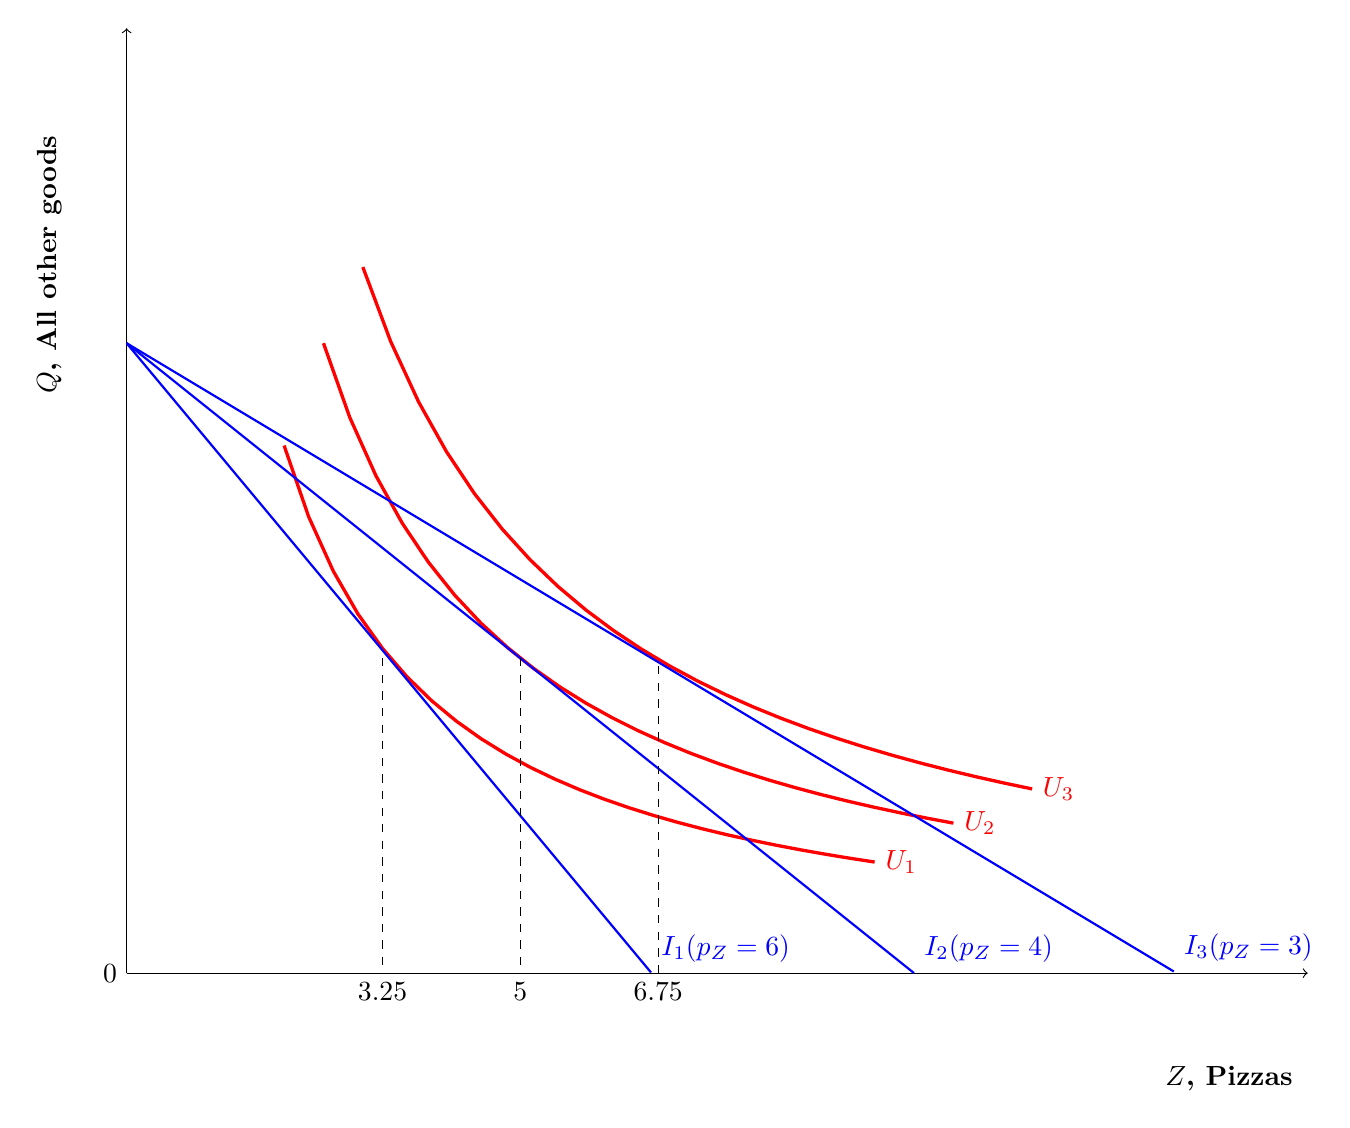
\begin{tikzpicture}
	\usetikzlibrary{calc}% Draw axes
	%Y
	\draw[->] (0,0) -- (0,12) ;
	\draw[] (0,8) -- node[rotate=90, above=20pt] {\textbf{$Q$, All other goods}} (0,10);
	%X
	\draw[->] (0,0) -- (15,0);
	\draw[] (14,0) -- node[below=30pt] {\textbf{$Z$, Pizzas}} (14,0);

	%Plot Indifference Curves
	%P=6
	\draw[color=red, very thick, domain=2:9.5] plot (\x,{(13.4/(\x))}) node[right] {{$U_{1}$}};
	%P=4
	\draw[color=red, very thick, domain=2.5:10.5] plot (\x,{(20/(\x))}) node[right] {{$U_{2}$}};
	%P=3
	\draw[color=red, very thick, domain=3:11.5] plot (\x,{(26.9/(\x))}) node[right] {{$U_{3}$}};

	%Plot Budget Constraint
	%P=6
	\draw[color=blue, thick, domain=0:6.66] plot (\x,{(40/5)-(6/5)*\x}) node[above right] {{$I_{1} (p_{Z}=6)$}};	
	%P=4
	\draw[color=blue, thick, domain=0:10] plot (\x,{(40/5)-(4/5)*\x}) node[above right] {{$I_{2} (p_{Z}=4)$}};
	%P=3
	\draw[color=blue, thick, domain=0:13.3] plot (\x,{(40/5)-(3/5)*\x}) node[above right] {{$I_{3} (p_{Z}=3)$}};
%	

	\draw[dashed] (5,4) -- (5,0);
	\draw[dashed] (3.25,4) -- (3.25,0);
	\draw[dashed] (6.75,3.9) -- (6.75,0);

	%Add axes labels
	%Origin%
	\node at (0,0) [left] {{0}};
	%Y Axis
%	\node at (0,8) [left] {{$Y/p_{B}=8$}};
%	\node at (0,4) [left] {{$4$}};
	%X Axis
	\node at (3.25,0) [below] {{$3.25$}};
	\node at (5,0) [below] {{$5$}};
	\node at (6.75,0) [below] {{$6.75$}};

	\end{tikzpicture}
	\begin{tikzpicture}
	\usetikzlibrary{calc}% Draw axes
	%Y
	\draw[->] (0,0) -- (0,12) ;
	\draw[] (0,8) -- node[rotate=90, above=20pt] {\textbf{$p_{Z}$, Price of Pizza}} (0,10);
	%X
	\draw[->] (0,0) -- (15,0);
	\draw[] (14,0) -- node[below=30pt] {\textbf{$Z$, Pizzas}} (14,0);

	\draw[very thick, red] plot[smooth, tension=.7] coordinates {(2,10) (3.25,6) (5,4) (6.75,3) (10,2)} node[right] {{$D$, Demand for Pizza}};

	\draw[dashed] (0,4) -- (5,4) -- (5,0);
	\draw[dashed] (0,6) -- (3.25,6) -- (3.25,0);
	\draw[dashed] (0,3) -- (6.75,3) -- (6.75,0);

	%Add axes labels
	%Origin%
	\node at (0,0) [left] {{0}};
	%Y Axis
	\node at (0,6) [left] {{$6$}};
	\node at (0,4) [left] {{$4$}};
	\node at (0,3) [left] {{$3$}};
	%X Axis
	\node at (3.25,0) [below] {{$3.25$}};
	\node at (5,0) [below] {{$5$}};
	\node at (6.75,0) [below] {{$6.75$}};


\end{tikzpicture}
}
\caption{Deriving Demand Curves}
\end{figure}
}

\section{Deviations from the Theory}

\frame{
	\frametitle{Deviations from the Theory: Behavioural Economics}
	\begin{itemize}
	\item Standard theory of consumer choice assumes that individuals are rational and seek to maximize their utility.
	\item[]
	\item Behavioural economics seeks to understand the implications of departures from these assumptions using insights from psychology, and empirical research on our cognitive and emotional biases.
	\item[]
	\item Goal: Refine the standard model to better predict economic decision making.
	\item[]
	\item Three key findings:
		\begin{enumerate}
		\item Transitivity
		\item Endowment effects
		\item Salience
		\end{enumerate}
	\end{itemize}
}

\frame{
	\frametitle{Deviations from the Theory: Transitivity}
	\begin{itemize}
	\item Key assumption of the standard model: preferences are transitive.
	\item[]
	\item Research suggests most adults exhibit transitivity for most economic decisions.
	\item[]
	\item Two cases where this finding fails:
			\begin{enumerate}
			\item Novel goods.
			\item Children.
			\end{enumerate}
	\item[]
	\item Do these failures matter?
	\end{itemize}
}

\frame{
	\frametitle{Deviations from the Theory: Endowment Effects}
	\begin{itemize}
	\item Standard model assumes that individuals value a good the same regardless of whether or not they own it.
	\item[]
	\item Empirical evidence suggests that most people place a higher value on a good if they own it then they do if they are considering buying it.
	\item[]
	\item Does this matter?
	\end{itemize}
}

\frame{
	\frametitle{Deviations from the Theory: Salience}
	\begin{itemize}
	\item Standard model assumes that individuals consider all possible information when making a decision.
	\item[]
	\item Empirical evidence suggests that people are more likely to consider information if it is presented in a way that grabs their attention, or if it takes relatively little thought or calculation to understand.
	\item[]
	\item Does this matter? How?
	\end{itemize}
}

\frame{
	\frametitle{Consumer Behaviour: Takeaways}
	\begin{enumerate}
	\item The theory of consumer choice is a model of consumer behaviour based on the idea that individuals make their consumption decisions to maximize their well being subject to the constraints that they face.
	\item[]
	\item The model can be use to predict consumer behaviour.
	\item[]
	\item While the model typically works very well, its usefulness can be limited by human psychology.
	\end{enumerate}
}

\end{document}
